% !TEX encoding = UTF-8 Unicode
% !TEX root = CCBusinessPlan.tex

\documentclass{book}

% !TEX root = SystemTemplate.tex

\usepackage[width=6.5in, height=9.2in, top=1.0in, papersize={8.5in,11in}]{geometry}
\usepackage[pdftex]{graphicx}
\usepackage{amsmath}
\usepackage{amsthm}
\usepackage{amssymb}
\usepackage[english]{babel}
\usepackage{tabularx}
%\usepackage{txfonts}
\usepackage{textcomp}
\usepackage{amsthm}
\usepackage[table]{xcolor}
\usepackage[margin=1in]{geometry}

\usepackage[all]{xy}
\usepackage{fancyhdr}
\pagestyle{fancy}
\usepackage{hyperref}
\usepackage{verbatim}
\usepackage{algorithm}
\usepackage{algorithmic}
\usepackage{array}
\usepackage{color}
\usepackage{listings}
\usepackage{calc}
\usepackage{doxygen}
\usepackage[utf8]{inputenc}
\usepackage{makeidx}
\usepackage{multicol}
\usepackage{multirow}
\usepackage[table]{xcolor}
\usepackage{tabularx}
\usepackage{framed}
\usepackage{xspace}
\usepackage{etex}
\usepackage{todonotes}
\usepackage{pdfpages}
\usepackage{pgfgantt}


%% Computer Modern Bright Font
%\usepackage{cmbright}
%\usepackage[T1]{fontenc}

%% Sans Serif Modern Font - similar to  Helvetica
\usepackage{lmodern}
\renewcommand*\familydefault{\sfdefault} %% Only if the base font of the document is to be sans serif
\usepackage[T1]{fontenc}


\definecolor{SDColor1}{rgb}{0,0,0}
\definecolor{SDColor2}{rgb}{0,0,0}
\definecolor{SDColor3}{rgb}{0,0,0}
\definecolor{SDColor4}{rgb}{0,0,0}
\definecolor{SDColor5}{rgb}{0,0,0}

%%%  --- Here are some other colors.  Keep it conservative --- %%%

%% Blue font color scheme
%\definecolor{SDColor1}{rgb}{.204,.353,.541}
%\definecolor{SDColor2}{rgb}{.31,.506,.741}
%\definecolor{SDColor3}{rgb}{0.18,0.35,0.59}
%\definecolor{SDColor4}{rgb}{0.44,0.59,0.82}
%\definecolor{SDColor5}{rgb}{0.35,0.35,0.35}
%

%% Brown color scheme
% \definecolor{SDColor1}{rgb}{.55,.2,.2}
%\definecolor{SDColor2}{rgb}{.4,.1,.1}
%\definecolor{SDColor3}{rgb}{.5, .15,.15}
%\definecolor{SDColor4}{rgb}{.63,.32,.18}
%\definecolor{SDColor5}{rgb}{.45,.15,.15}
%


%% Custom colors for code listing environment
\definecolor{OliveGreen}{cmyk}{0.64,0,0.95,0.40}
\definecolor{DarkBlue}{cmyk}{0.76,0.76,0,0.20}
\definecolor{DarkRed}{cmyk}{0,1,1,0.45}
\lstset{language=c,frame=ltrb,framesep=5pt,basicstyle=\normalsize,
 keywordstyle=\ttfamily\color{DarkRed},
identifierstyle=\ttfamily\color{DarkBlue}\bfseries,
commentstyle=\color{OliveGreen},
stringstyle=\ttfamily,
showstringspaces=false,tabsize = 3}


\setlength{\oddsidemargin}{0mm} 
\setlength{\evensidemargin}{0mm} 

%% Uncomment if you want "Draft" placed on each page.
%\usepackage{draftwatermark}
%\SetWatermarkLightness{0.975}
%\SetWatermarkScale{1}
%\SetWatermarkText{Draft}

\pagestyle{fancy}
\renewcommand{\chaptermark}[1]{\markboth{#1}{}}
\renewcommand{\sectionmark}[1]{\markright{\thesection\ #1}}
\fancyhf{}
\fancyhead[LE,RO]{\bfseries\thepage}
\fancyhead[LO]{\bfseries\rightmark}
\fancyhead[RE]{\bfseries\leftmark}
%\fancyfoot[LE,RO]{Confidential and Proprietary}
%\renewcommand{\headrulewidth}{0.5pt}
%\renewcommand{\footrulewidth}{0pt}
%\addtolength{\headheight}{0.5pt}
%\setlength{\footskip}{0mm}
%\renewcommand{\footruleskip}{0pt}



\usepackage{titlesec}
\titleformat{\chapter}[display]
{\normalfont\bfseries\color{SDColor3}}    %\normalfont\bfseries\filcenter}
{\LARGE\thechapter}
{1ex}
{\titlerule[2pt]
\vspace{2ex}%
\LARGE}
[\vspace{1ex}%
{\titlerule[2pt]}]

%
%\usepackage{titlesec}
%\titleformat{\chapter}{\normalfont\bfseries\LARGE}
%{\thechapter.}{5pt}{}[{\titlerule[3pt]}]
%
%\titleformat{\section}{\normalfont\bfseries\Large}
%{\thesection.}{5pt}{}[{\titlerule[2pt]}]
%
%\titleformat{\subsection}{\normalfont\bfseries\large}
%{\thesubsection.}{5pt}{}[{\titlerule[1pt]}]
%


%\titleformat*{\section}{\Large\bfseries\sffamily\color{SDColor1}}
%\titleformat*{\subsection}{\large\bfseries\sffamily\color{MSLightBlue}}
%\titleformat*{\section}{\Large\bfseries\color{SDColor3}}
%\titleformat*{\subsection}{\large\bfseries\color{SDColor4}}

%\titleformat*{\section}{\Large\bfseries}
%\titleformat*{\subsection}{\large\bfseries}
%\titleformat*{\subsubsection}{\large\bfseries}

\titleformat*{\section}{\Large\bfseries\color{SDColor1}}  
\titleformat*{\subsection}{\large\bfseries\color{SDColor2}}
\titleformat*{\subsubsection}{\large\bfseries\color{SDColor5}}
\setcounter{secnumdepth}{3}
\renewcommand{\thesubsubsection}{\thesubsection.\alph{subsubsection}}

% Save the original chapter command as stdchapter
\let\stdchapter\chapter

%redefine the backmatter command
\let\stdbackmatter\backmatter
\makeatletter% We need the '@' letter to call if@openright
\renewcommand{\backmatter}{
\stdbackmatter
% need to set the page counter back to 1
\setcounter{page}{1}
%% Redefine the \chapter command for our Back Matter
\renewcommand{\chapter}[1]{
  \if@openright\cleardoublepage\else\clearpage\fi% chapters begin on right page
  \stdchapter{##1}% output standard chapter heading
  \setcounter{section}{0}% restart the section numbering
  \renewcommand{\thepage}{BM-\arabic{page}}% Redefine page numbering format
  \renewcommand{\thesection}{\arabic{section}}% Redefine section number format
}}
\makeatother% Restore the normal behavior of '@'

%redefine the appendix command
\let\stdappendix\appendix
\makeatletter% We need the '@' letter to call if@openright
\renewcommand{\appendix}{
\stdappendix
%% \titleformat{\chapter}[display]
%% {\normalfont\bfseries\color{SDColor3}}    %\normalfont\bfseries\filcenter}
%% {\LARGE Appendix \thechapter}
%% {1ex}
%% {\titlerule[2pt]
%% \vspace{2ex}%
%% \LARGE}
%% [\vspace{1ex}%
%% {\titlerule[2pt]}]
  %%% Since counters are different in the appendix section
  %%% we redefine \chapter to explicitly reset the page number
  %%%  (comment out to see effect)
  \renewcommand{\chapter}[1]{
    \stdchapter{##1}\setcounter{page}{1}
    %%% We also redefine page numbering
    \renewcommand{\thepage}{\Alph{chapter}-\arabic{page}}
  }
}
\makeatother% Restore the normal behavior of '@'


\makeatletter% We need the '@' letter to call if@openright
\newcommand{\agreement}{
  \renewcommand{\chapter}[1]{
    \if@openright\cleardoublepage\else\clearpage\fi% chapters begin on right page
    \pagestyle{plain}% turn off fancy headers
    \setcounter{section}{0}% Reset the section number
    \setcounter{page}{1}% Reset the page number
    \renewcommand{\thepage}{SA-\arabic{page}}% Set format for page numbering
    \renewcommand{\thesection}{\arabic{section}}% Set format for section numbering
    \refstepcounter{chapter}% Add it to the index/toc for on-line viewing
    \addcontentsline{toc}{chapter}{##1}% Add to the table of contents
  }
}
\makeatother% Restore the normal behavior of '@'



%%  If you do some math typesetting, you may want more environment names.
%% Uncomment to see how this works:
%\newtheorem{summary}{Summary:}
%\newtheorem{example}{Example:}



 % This sets the format.

% Add your title page contents here 
\title{{\color{SDColor3} \rule{\linewidth}{0.5mm}}\\[2mm] {\huge \bfseries \color{SDColor3} CrowdControl }\\[-1mm] {\color{SDColor3}\rule{\linewidth}{0.5mm}} \\  \vfill
{\LARGE \bfseries \color{SDColor4} Business Plan }\\  \vfill 
{\color{SDColor3} Bowtaps} }
\author{\color{SDColor3} Charles Bonn \and \color{SDColor3} Johnathan Ackerman \and  \color{SDColor3} Daniel Andrus \and  \color{SDColor3}Evan Hammer \and  \color{SDColor3} Joseph Mowry }
\date{\color{SDColor3} \today}


\begin{document}

\frontmatter

\addcontentsline{toc}{chapter}{Title}
\maketitle
\tableofcontents
\addcontentsline{toc}{chapter}{Contents}


%\chapter{Overview Statements}
%% !TEX root = DesignDocument.tex

\section{Mission Statement}
Mission statement inserted here.   

\section{Elevator Pitch}
Elevator Pitch inserted here.   
  % add mission statement to mission.tex

%\chapter{Document Preparation and Updates}
%% !TEX root = DesignDocument.tex



Current Version [1.5.3]
\vspace*{5mm}

{\color{SDColor5}
\noindent
\textit{Prepared By:}\\
\textit{Johnathan Ackerman}\\
\textit{Daniel Andrus}\\
\textit{Charles Bonn}\\
\textit{Evan Hammer}\\
\textit{Joseph Mowry}
}
\vfill
\noindent
{\color{SDColor3} \textit{\textbf{Revision History}}}\\
\begin{tabular}{|>{\raggedright}p{1.5cm}|>{\raggedright}p{3cm}|>{\raggedright}p{1.5cm}|>{\raggedright}p{9cm}|}
\hline
\textit{\textbf{Date}} &  \textit{\textbf{Author}} & \textit{\textbf{Version}} & \textit{\textbf{Comments}}\tabularnewline
\hline
 \textit{\textbf{10/1/15}} & \textit{Charles Bonn} & \textit{1.0.0} & \textit{Sprint 1 \& Senior Design Contract}\tabularnewline
 \hline
  \textit{\textbf{11/3/15}} & \textit{Charles Bonn} & \textit{1.1.0} & \textit{Sprint 2 Documentation}\tabularnewline
 \hline
 \textit{\textbf{12/11/15}} & \textit{Charles Bonn} & \textit{1.2.0} & \textit{Sprint 3 finished, résumés added}\tabularnewline
\hline
 \textit{\textbf{1/15/16}} & \textit{Daniel Andrus} & \textit{1.2.1} & \textit{iOS documentation added}\tabularnewline
\hline
 \textit{\textbf{1/18/16}} & \textit{Joseph Mowry} & \textit{1.3.0} & \textit{Winter Sprint Report added}\tabularnewline
\hline
 \textit{\textbf{2/12/16}} & \textit{Charles Bonn} & \textit{1.4.0} & \textit{Sprint 4 Report, general content added}\tabularnewline
\hline
 \textit{\textbf{2/18/16}} & \textit{Joseph Mowry} & \textit{1.5.0} & \textit{Sprint 5 Report, various chapter revisions}\tabularnewline
\hline
 \textit{\textbf{2/19/16}} & \textit{Charles Bonn} & \textit{1.5.1} & \textit{Sprint 5 Report, organizational changes, chapter revisions}\tabularnewline
\hline
 \textit{\textbf{2/24/16}} & \textit{Johnathan Ackerman} & \textit{1.5.2} & \textit{Overview rewrite}\tabularnewline
\hline
 \textit{\textbf{3/17/16}} & \textit{Evan Hammer} & \textit{1.5.3} & \textit{Document cleanup, organizational changes}\tabularnewline
\hline
\textit{\textbf{4/29/16}} & \textit{Johnathan Ackerman} & \textit{1.6.0} & \textit{Completed Chapter 6}\tabularnewline
\hline
\textit{\textbf{4/22/16}} & \textit{Joeseph Mowry} & \textit{1.6.1} & \textit{Completed Chapters 0, 1}\tabularnewline
\hline
\textit{\textbf{4/30/16}} & \textit{Evan Hammer} & \textit{1.6.2} & \textit{Completed Chapters 2, 3}\tabularnewline
\hline
\textit{\textbf{5/2/2016}} & \textit{Joeseph Mowry} & \textit{1.6.3} & \textit{Completed Chapter 4}\tabularnewline
\hline
\textit{\textbf{5/2/2016}} & \textit{Charles Bonn} & \textit{1.6.4} & \textit{Completed Chapters 8, 9, 10}\tabularnewline
\hline
\textit{\textbf{5/2/2016}} & \textit{Johnathan Ackerman} & \textit{1.6.5} & \textit{Completed Chapter 7}\tabularnewline
\hline
\textit{\textbf{5/3/2016}} & \textit{Dan Andrus} & \textit{1.6.6} & \textit{Completed Chapter 5}\tabularnewline
 &  &  & \tabularnewline
\hline
\end{tabular}
\vfill


 
\mainmatter

%% The term "cleaning" used in the syllabus means removing all of the sample content I
%% have provided.   You can comment out by using the comment character or the comment
%% environment.  

%%  Add to the following chapters

% !TEX root = CCBusinessPlan.tex

\chapter{Executive Summary}

Bowtaps is a software development company focused on technological innovation. We aim to provide mobile solutions that alleviate the stresses of modern life. Our passionate and experienced developers strive to create products that will change the way users go about their daily lives.\\

Our flagship product is Crowd Control, a mobile application designed to ease the experience of going out. Crowd Control will accomplish this through integrated group messaging, GPS mapping, and group status updates. It will provide users with a reliable and easy way to track their friends and fellow users at events of any kind, while providing local businesses a platform to showcase their venue.\\
 
Currently there is nothing on the market that meets the same set of needs that we are targetting. As we will detail later on, other existing services only implement one key aspect of our app whereas Crowd Control brings all of these core features together into a single product.\\
 
Our initial market entry plan is to keep the app free to download in order to lower the barrier of entry for users. Sponsored ads, or “suggestions”, will be our primary revenue source. Suggestions are a way to give users ideas for possible events for their group to attend in their area.\\

Ad space will be priced based on the population of users in the area. Since this price is essentially demand-driven, advertisement prices will be calculated based on user growth in the area. It is important to note that our advertisements are not traditional banner ads; rather, they are sponsored event suggestions made available to users that are searching for events in their area. We believe this is especially attractive to users as it is unobtrusive while adding value and content. Advertisers would also benefit from our unique approach to advertising as it would entice more impressions from users.\\

In the app market, the entry into the marketplace is crucial, especially as a start-up company. Currently, without other released products to generate revenue, it is important that user base grow as quickly as possible. A strong entry into the marketplace will help fuel further development and allow us to expand Crowd Control with additional features. Targetting local high-traffic events as our beachhead markets will aid in early growth and provide us the insight needed to plan expansion to new markets.\\

As our user base dictates our finances, our goal is to minimize development costs up until the launch of Crowd Control. To accomplish this, all backend services we utilize implement a scalable pricing plan that is free for low usage amounts. As our usage exceeds one million unique server requests per month, costs will increase and must be maintained in the release phase. Additionally, Crowd Control was programmed in such a way that, if needed, we can transition away from our current back-end services with relative ease.
  
% !TEX root = CCBusinessPlan.tex


\chapter{General Company Description}


\section{Company Summary}

BowTaps is a software development company focused on a complete user experience. The company founded the mobile application Crowd Control. As a start-up company we have a close connected group of people that have the shared goals of changing how people use mobile applications for the better

\section{Mission}

Our mission at BowTaps is to develop innovative mobile software applications to provide solutions to inconveniences that trouble the everyday user. With our software we plan on changing the mobile environment by creating applications with easy to use and  intuitive interfaces with reliable services for everyday use.

\section{Objectives}

	\begin{itemize}
	\item Generate revenue
	\item Provide users with value added user-friendly applications
	\end{itemize}


\section{Keys To Success}

	\begin{itemize}
	\item High quality and innovative development skills
	\item Strategic planning 
	\item Rapidly gaining users and maintaining growth 
	\item Reliable technology
	\end{itemize}

\section{Company History}

Our team consists of five employees made up of undergraduate Computer Science students from the South Dakota School of Mines & Technologies. 

Charles Bonn: Charles Bonn founded the idea of a mobile application that would help locate and manage groups of people; this idea grew into Crowd Control. As the CEO and Project Manager, Charles acts as the intermediary between BowTaps and the Community of app development. On the technical side he is working with the server backend and communication of the server and Crowd Control 
Johnathan Ackerman: Johnathan is designated as our Quality Assurance specialist. He would be responsible for fact-checking the group’s work and ensuring that the project fits within design specifications and complies with coding standards. During development for Crowd Control, he will also contribute as the lead Graphical designer for android and create the android user interface experience.
Daniel Andrus: 
Our Lead Designer, Daniel, is responsible for creating an adaptive and attractive user experience for Crowd Control. He will also be with collaborating with Evan Hammer and Charles Bonn on product and company branding. As development begins he will be working with the iOS user interface experience.
Evan Hammer: In charge of Sales and Marketing information, Evan keeps track of and coordinates expense and revenue flow related to the company. Evan also provides a unique and useful perspective on our target demographic with his prior job experience. He will work with local businesses and events both to promote our product and to advertise on our platform. As development begins he will be concentration on creating the backend for iOS. 
Joseph Mowry: Joseph is in charge of designing the data models supporting Crowd Control. With the database being a key feature he will design and implement key features that will allow Crowd Control to be a versatile and efficient application. As development begins he will be concentrating on the backend of Android development.







% !TEX root = CCBusinessPlan.tex


%\setlist{nolistsep}
\definecolor{green}{HTML}{66FF66}
\definecolor{myGreen}{HTML}{009900}

\renewcommand{\familydefault}{\sfdefault}
\renewcommand{\arraystretch}{1.5}

\chapter{The Product}

\section{Introduction}

Crowd Control is a mobile application designed to “ease the experience of going out.” Crowd Control seeks to provide users involved in nightlife events, concerts, festivals, and any other group activities, mobile technology to add value to their overall experience. 

\section{Third Party Requirements}

This application is designed to be a background tool. It has to handle importing and exporting messaging and GPS data to and from the user. It has to keep this information up-to-date as well as quickly accessible. It also has to store this information in a safe and secure way.
For the side being developed in Android. We have handled the following problems though the use of services, and the UX design of the app. For storing the information, we are using a back-end service called Parse. Parse encrypts all of its data and gives great functionality to a database. Another service being used for the messaging, Sinch. Sinch also uses encryption to protect app-to-app messages.
The goal of our UX is to make it so that the user the doesn't have to think about the about. We accomplish this by implementing a one-time log in for the user. Another way we will be streamlining things is by keeping the app at the group screen when launched when the user is in said group.\\

\noindent
\textbf{Parse}

Parse is a back-end database service that is the backbone of this app. The entirety of its database is encrypted for our users protection. Inside Parse we are using several tables. These tables abstract user information so that even the displayed information is limited to protect the user.\\

\noindent
\textbf{Sinch}

Sinch is a back-end messaging system. It provides encrypted device-to-device messaging. Though sinch, we will be able to maintain a more stable messaging platform.




\section{Developement Requirements}

An important question we need to ask ourselves right away is what type of application we want to develop. The two basics types to choose from are a native version and a cross platform development.  The following information pulled directly from uxmag.com will outline the differences, strengths, and drawbacks of both types.
A native app is one that is built for a specific platform, such as iPhone or Android, using their code libraries and accessing their available hardware features (camera, GPS, etc). A cross platform compiler, such as Xamarin, allows for simultaneous development on both platforms but does have its drawbacks.. Let's explore the pros and cons of both approaches.



\begin{center}
\begin{tabularx}{\textwidth}[t]{m{4cm} X}
%table spot one
\arrayrulecolor{green}\hline
\textbf{\textcolor{myGreen}{Native App Strengths}} & \\
\hline
Speed.  &
\begin{minipage}[t]{\linewidth}%
\begin{itemize}
\item[1.1] 
Native apps tend to be faster and more responsive. Because the code that runs the app is stored locally on the phone, there is no time spent waiting for static content (such as images and text) to be downloaded from the web. While dynamic content may still need to be accessed from the web, it’s an improvement over the web-based model in which everything needs to be downloaded each time.\\

\end{itemize} 
\end{minipage}\\

\arrayrulecolor{black}\hline

Local Storage &
\begin{minipage}[t]{\linewidth}%
\begin{itemize}
\item[1.2] Native apps can run asynchronously, meaning dynamic information can be stored locally on the phone temporarily and synced with the central web-based server later. While new technologies and features (such as those in Xamarin) will allow for this to also be done in cross platform environment it is not as reliable as native.\\
\end{itemize} 
\end{minipage}\\

\hline

Killer Features &
\begin{minipage}[t]{\linewidth}%
\begin{itemize}
\item[1.3]  Going with the native app approach gives you access to that platform's hardware features allowing interesting functionalities such as taking photos, accessing GPS information, making phone calls, leveraging near field communication (NFC), etc. Because web-based apps are platform agnostic, they do not have access to the device’s hardware features.\\
\end{itemize}
\end{minipage}\\

% section 2
\arrayrulecolor{green}\hline
\textbf{\textcolor{myGreen}{Native App Draw Backs}} \\
\hline

Coding &
\begin{minipage}[t]{\linewidth}%
\begin{itemize}
\item[2.1] The biggest drawback to developing a native app vs. a cross platform one is that a separate code base must be created and maintained for each individual platform. For example, if you decided to initially build an iPhone app, you would have to design, code, and deploy an iOS app to the App Store. If you then decide down the road that you also want an Android version, you will have to redesign the app for the Android device, code and deploy it to the Android app store—likewise for other platforms. From a development perspective, the code bases are two entirely different languages and will have to be completely rewritten simply to mimic the original app’s functionality.\\
\end{itemize}
\end{minipage}\\

% section 3
\hline
\multicolumn{2}{l}{%
\textbf{\textcolor{myGreen}{Cross Platform Strengths}}} \\
\hline

Single Solution &
\begin{minipage}[t]{\linewidth}%
\begin{itemize}
\item[3.1] The biggest upside to a cross platform development approach is, of course, the biggest downside to a native one. When developing a cross platform you are centralizing your offering. Single-source means that there is a single version of the code base that all users across all platforms access and use.\\
\end{itemize} 
\end{minipage}\\

Single Code Updates &
\begin{minipage}[t]{\linewidth}%
\begin{itemize}
\item[3.2] With the language being written in a single language allows for faster updates and new features to be added.  \\
\end{itemize} 
\end{minipage}\\



%section 4
\hline
\multicolumn{2}{l}{%
\textbf{\textcolor{myGreen}{Cross Platform Draw Backs}}} \\
\hline

Hardware &
\begin{minipage}[t]{\linewidth}%
\begin{itemize}
\item[3.1] With cross platform development does not always properly implement the features of the native language. For the things that require specific native code you have to create translators to go between the cross code and the native code.
\end{itemize} 
\end{minipage}\\


\end{tabularx}
\end{center}

\noindent
\textbf{Our Decision}

Both approaches certainly have their share of benefits as well as drawbacks. A long-term strategy would seem to favor web-based over native apps, but no matter which approach is taken, a well-orchestrated user experience is the best defense in the rapidly evolving world of mobile platforms and devices. We have decided to use the native approach because it allows for a more 

\section{Product Description}

Crowd Control is a mobile application, which aims to add value to the overall experience of event goers though group management, integrated group messaging, and gps locations. All of these features will be bundled into a easy to use mobile application that allows for everything your group needs to know to be in one location at all times.

\subsection{Overview}

The application was built to serve three primary aspects of crowd control: 
\begin{itemize}
\item Event-based group management
\item Integrated group chat
\item Opt-in periodic location updates
         (Detailed)
\end{itemize}

\subsection{Features}

\textit{\textbf{Group Management:}}\\

The application will allow users to create temporary groups with known and unknown users. The groups will disband after an event is over, allowing a more dynamic experience. \\

\noindent
\textit{\textbf{Group Messaging:}} \\

The mobile application will feature an integrated messenger, which removes the need for users to resort to third-party services to communicate with group members. Along with third party messaging apps ( ones that are outside of the app ) it allows for ease because it eliminates the issues associated with group messaging such as, cross platform messaging, cross carrier messaging, and time stamping issues. \\

\noindent
\textit{\textbf{GPS Tracking:}}\\

Many third-party applications use the GPS feature to help track other users. Our GPS tracking is designed with groups and battery life in mind. Our implementation would be less demanding on the users’ batteries by only sending location updates at customizable time intervals or when requested. Because the groups are temporary, tracking stops after the group is disbanded. \\








%\bibliographystyle{plain}
%\bibliography{designrefs.bib}
%\addcontentsline{toc}{chapter}{Bibliography}


% We want to add the Software agreement to the end and number the
% pages separately from the document.  We don't want to do a standard
% chapter heading, but we do want it to appear in the table of contents
% and in the index used for on-line viewing.  We defined the \agreement
% macro to set things up for us.
%\agreement

%\chapter{Software Agreement}
%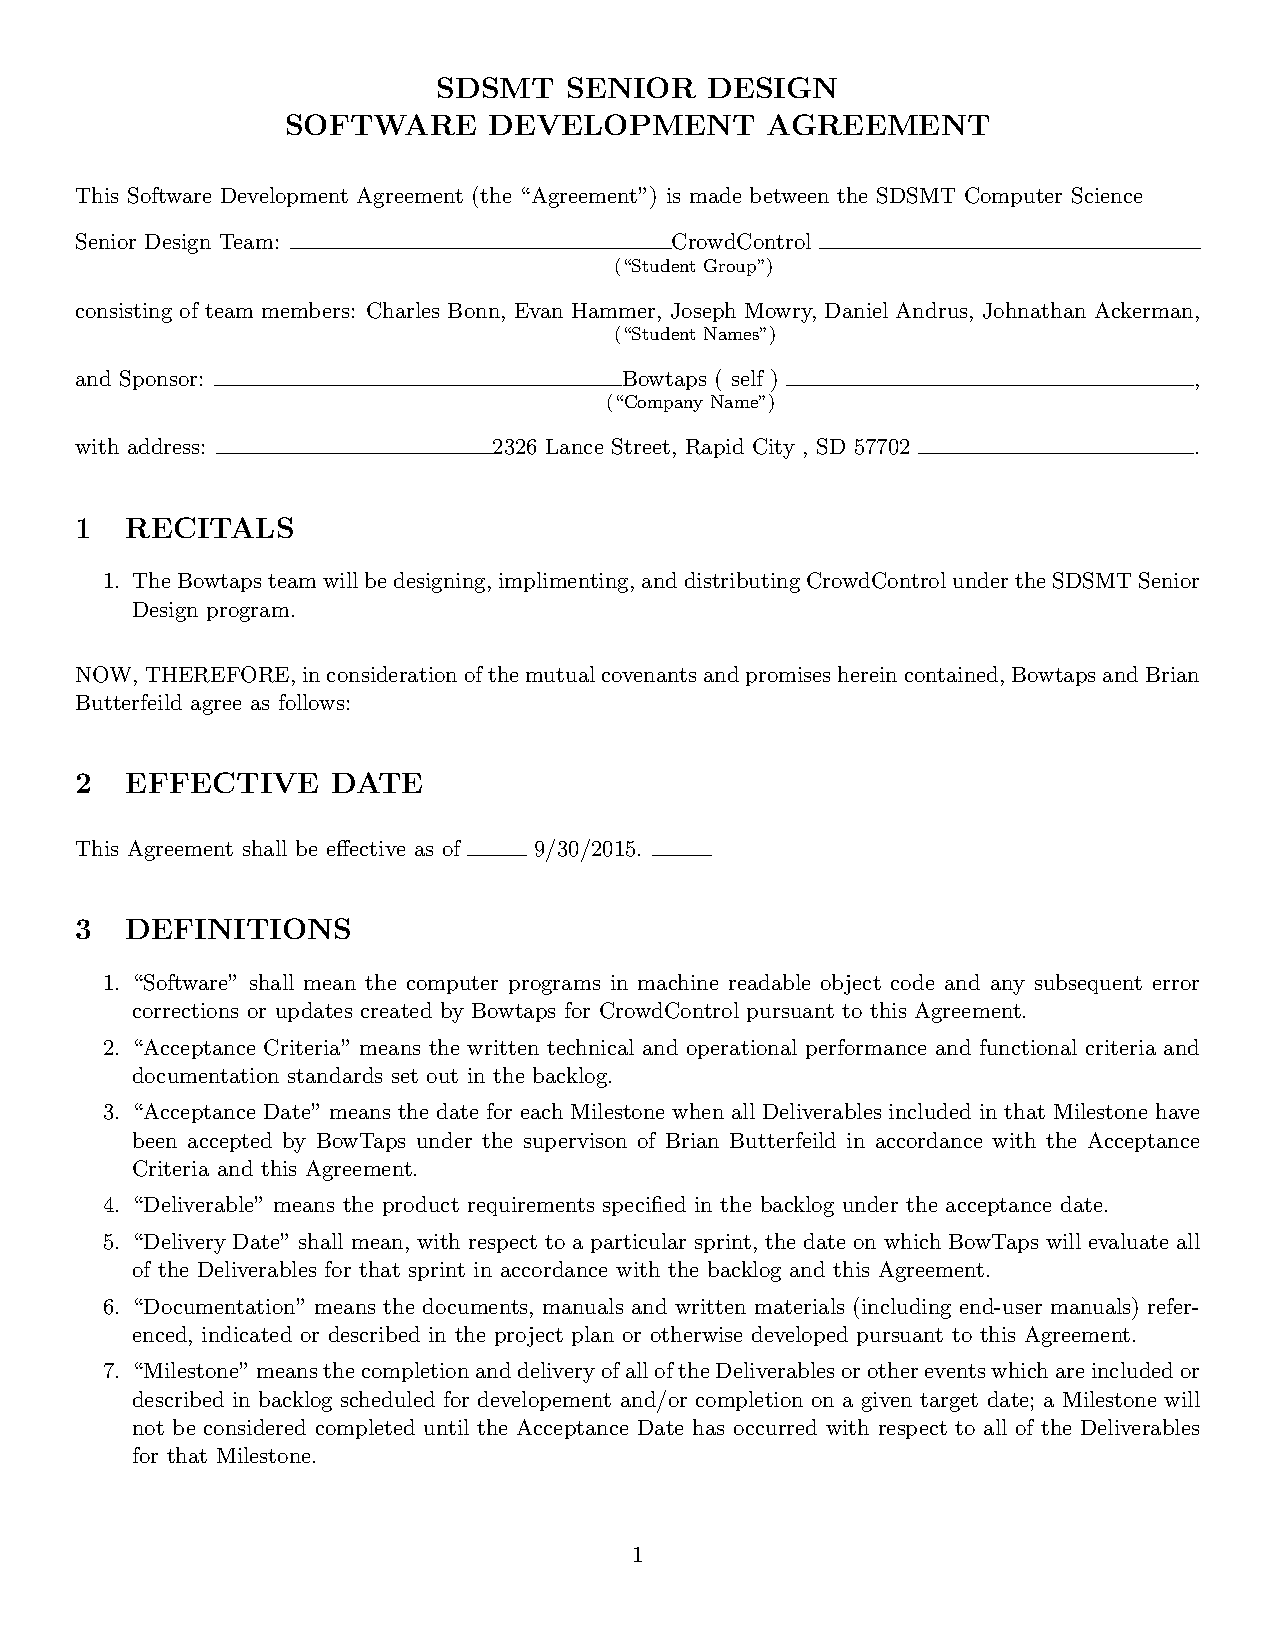
\includepdf[pages={1-5}]{SoftwareContract.pdf}

% In our style file, appendices are numbered with capital letters
%\appendix

%\chapter{Product Description}
%% !TEX root = DesignDocument.tex


%Write a description of the product to be developed.
%Use sectioning commands as neccessary.
%\vspace{2\baselineskip}

%\centerline{\Large {\bf NOTE:} {\em This is part of the contract.}}

CrowdControl is a group management application that will be an application that has gps features, group messaging, group management features.

\section{GPS Features}

\subsection{Group Members}

The Group member gps features will allow for users to track other users in the same group as they are. This will be under user permission to allow other user to see there location.

\subsection{Suggestions}

The suggestion side of the GPS will take a user or group location and give even suggestions of places to go or things to do in the area of the group.

\section{Group Messaging}

Integrated group messaging on a single platform uniform to iOS and android. 

\section{Group Manangement Features}

This will allow for members to join a group, add a member to a group, and leave a group.

\section{Parse Features}

Parse will be used to store user data and group data.


%\chapter{Publications}   %% Research track 
%% !TEX root = SystemTemplate.tex


Research Track:  
This chapter will include any publications generated from the research.  Most likely these will be preprints and one will just include the pdf.

%\includepdf[pages={1-5}]{Pub1.pdf}



%\chapter{Sprint Reports}
%% !TEX root = DesignDocument.tex


%\section{Sprint Report \#1}

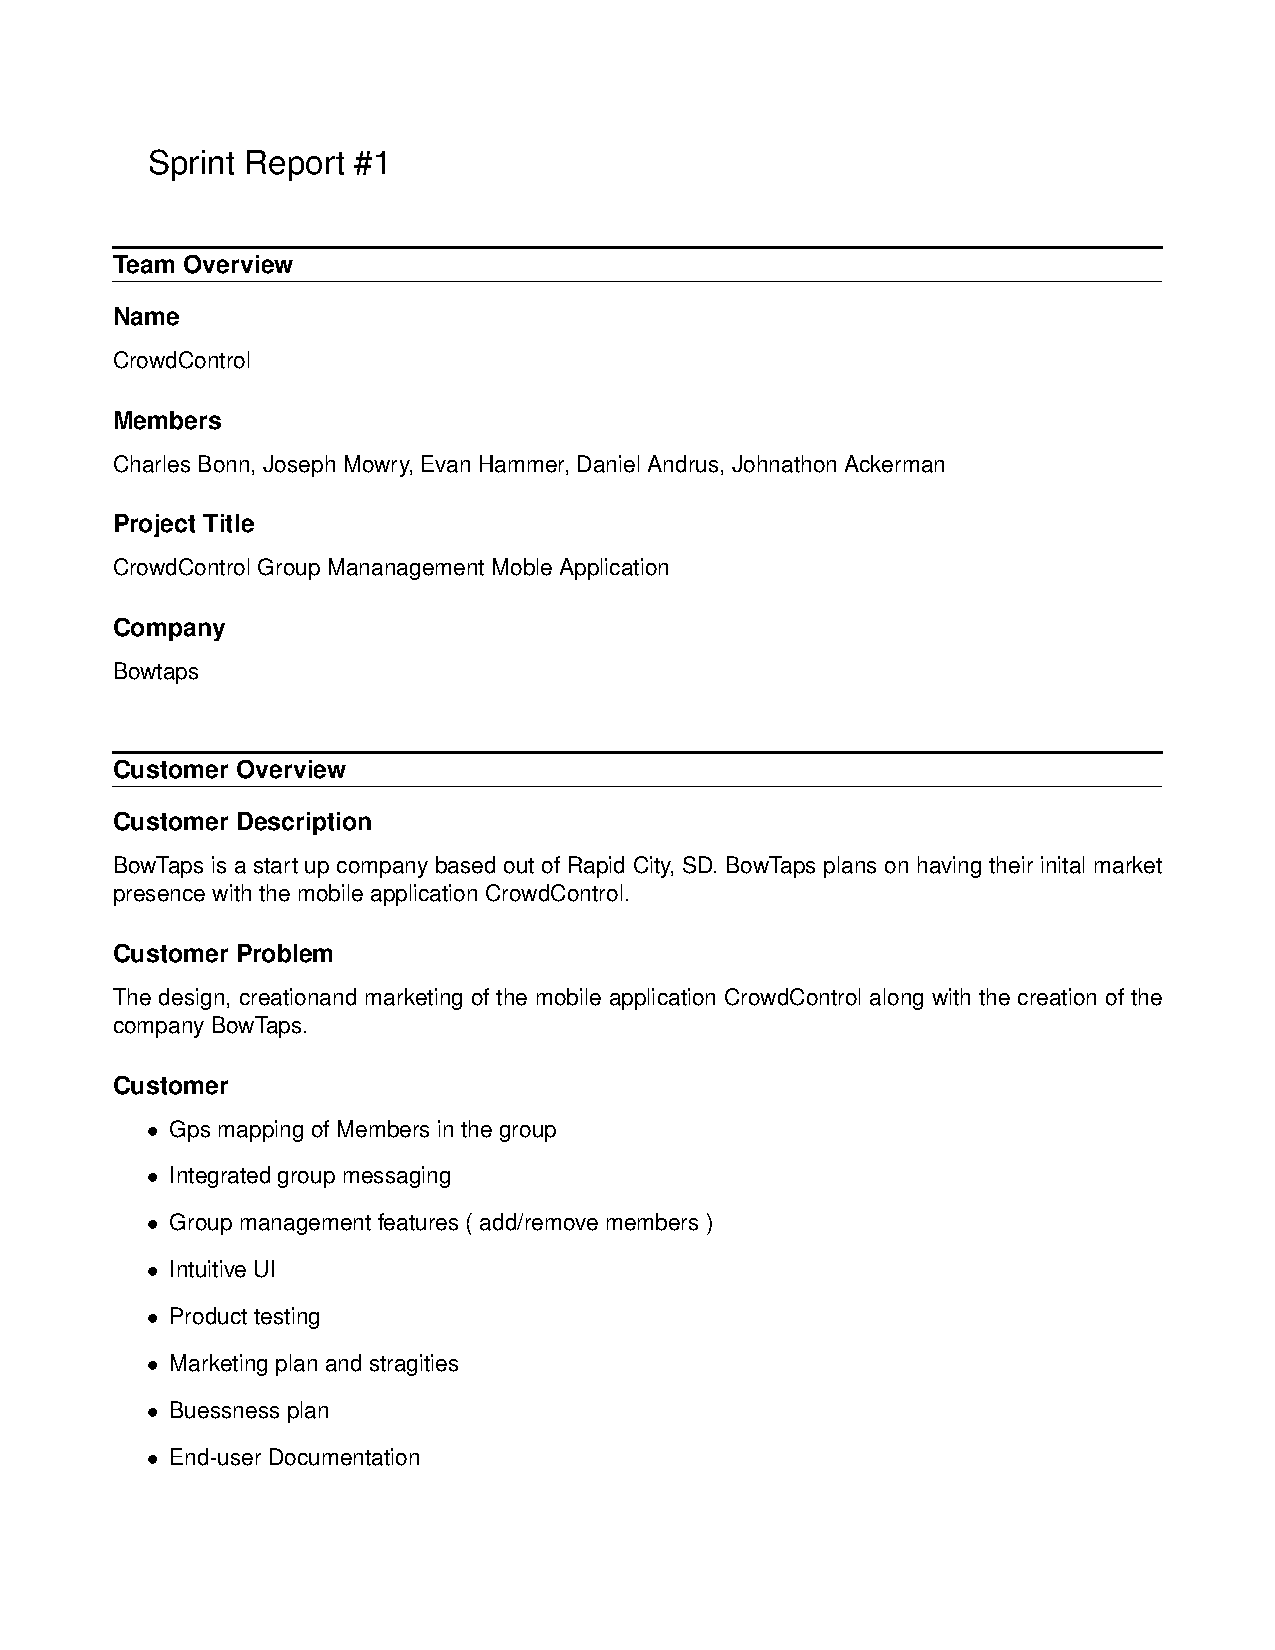
\includepdf[pages=-]{Additional/sprints/sprint1_wrapper.pdf}

%\section{Sprint Report \#2}

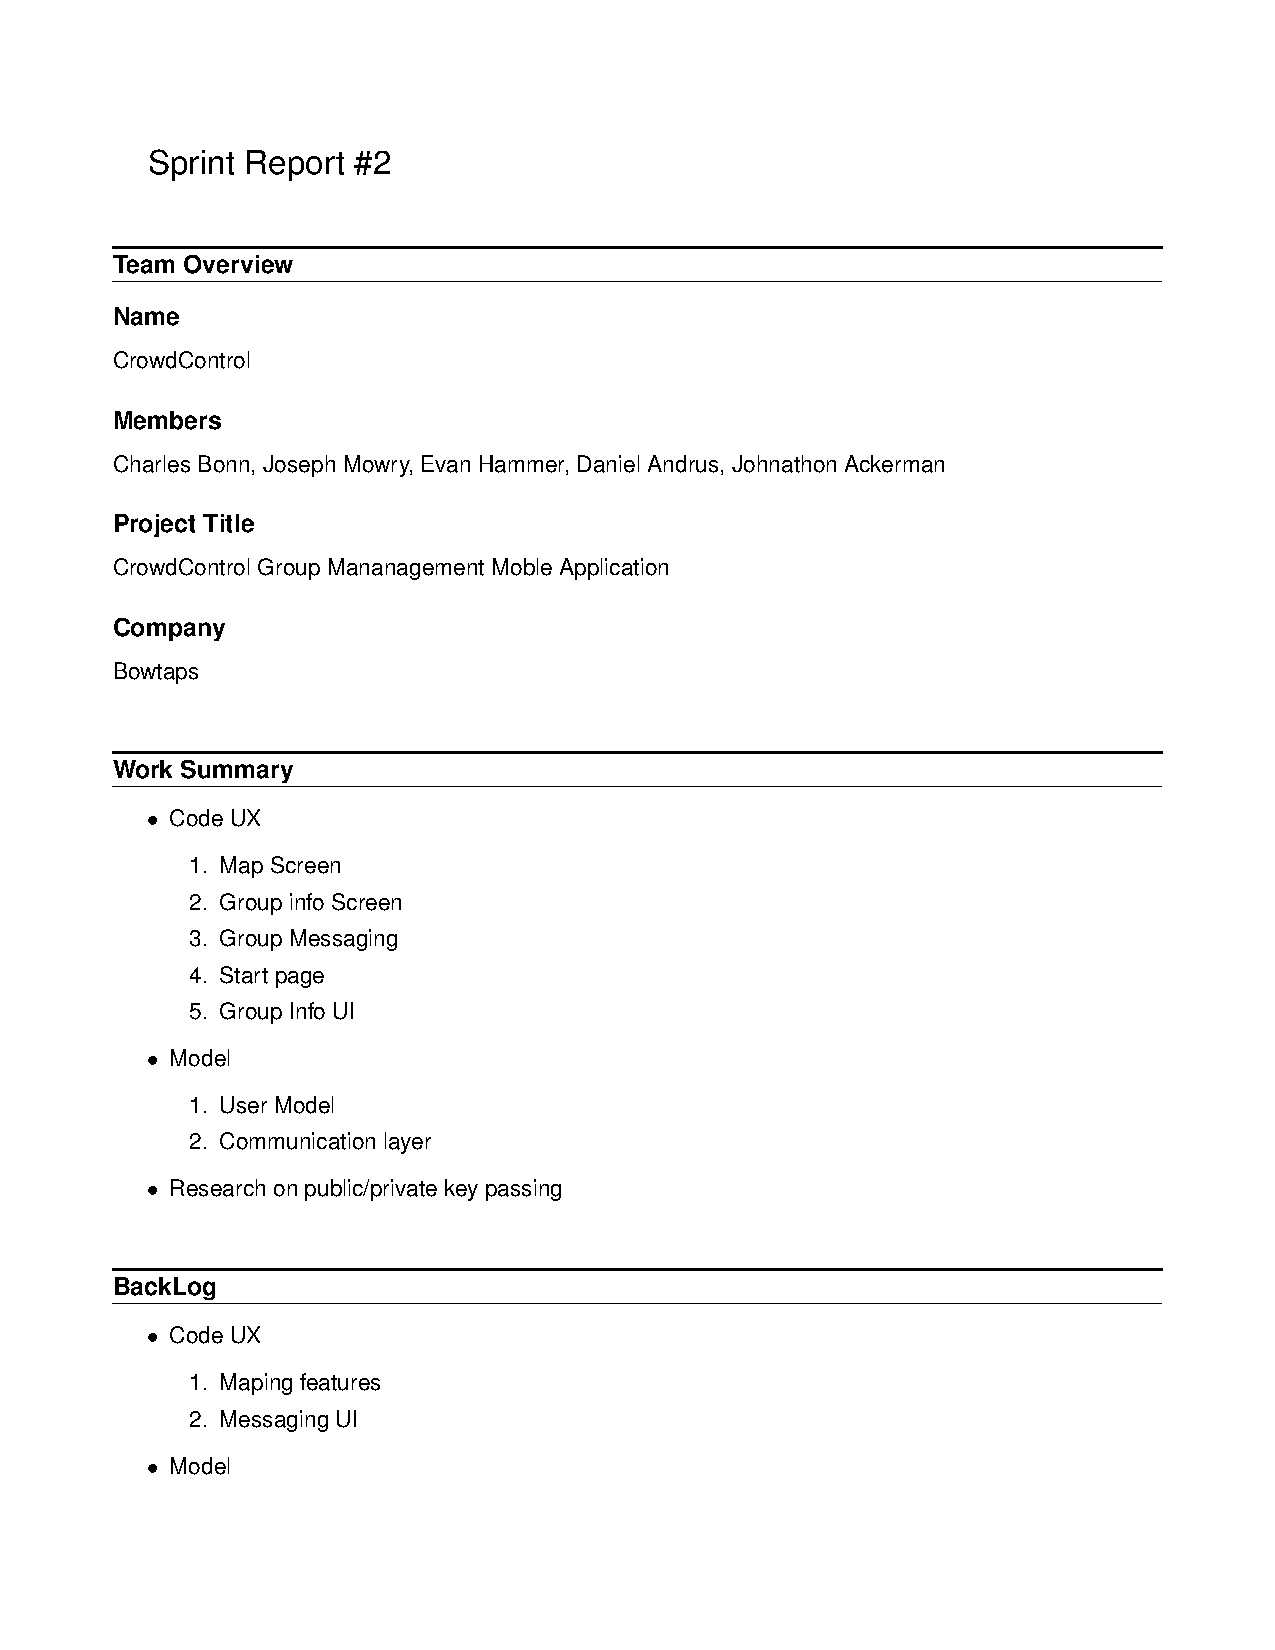
\includepdf[pages=-]{Additional/sprints/sprint2_wrapper.pdf}

%\section{Sprint Report \#3}

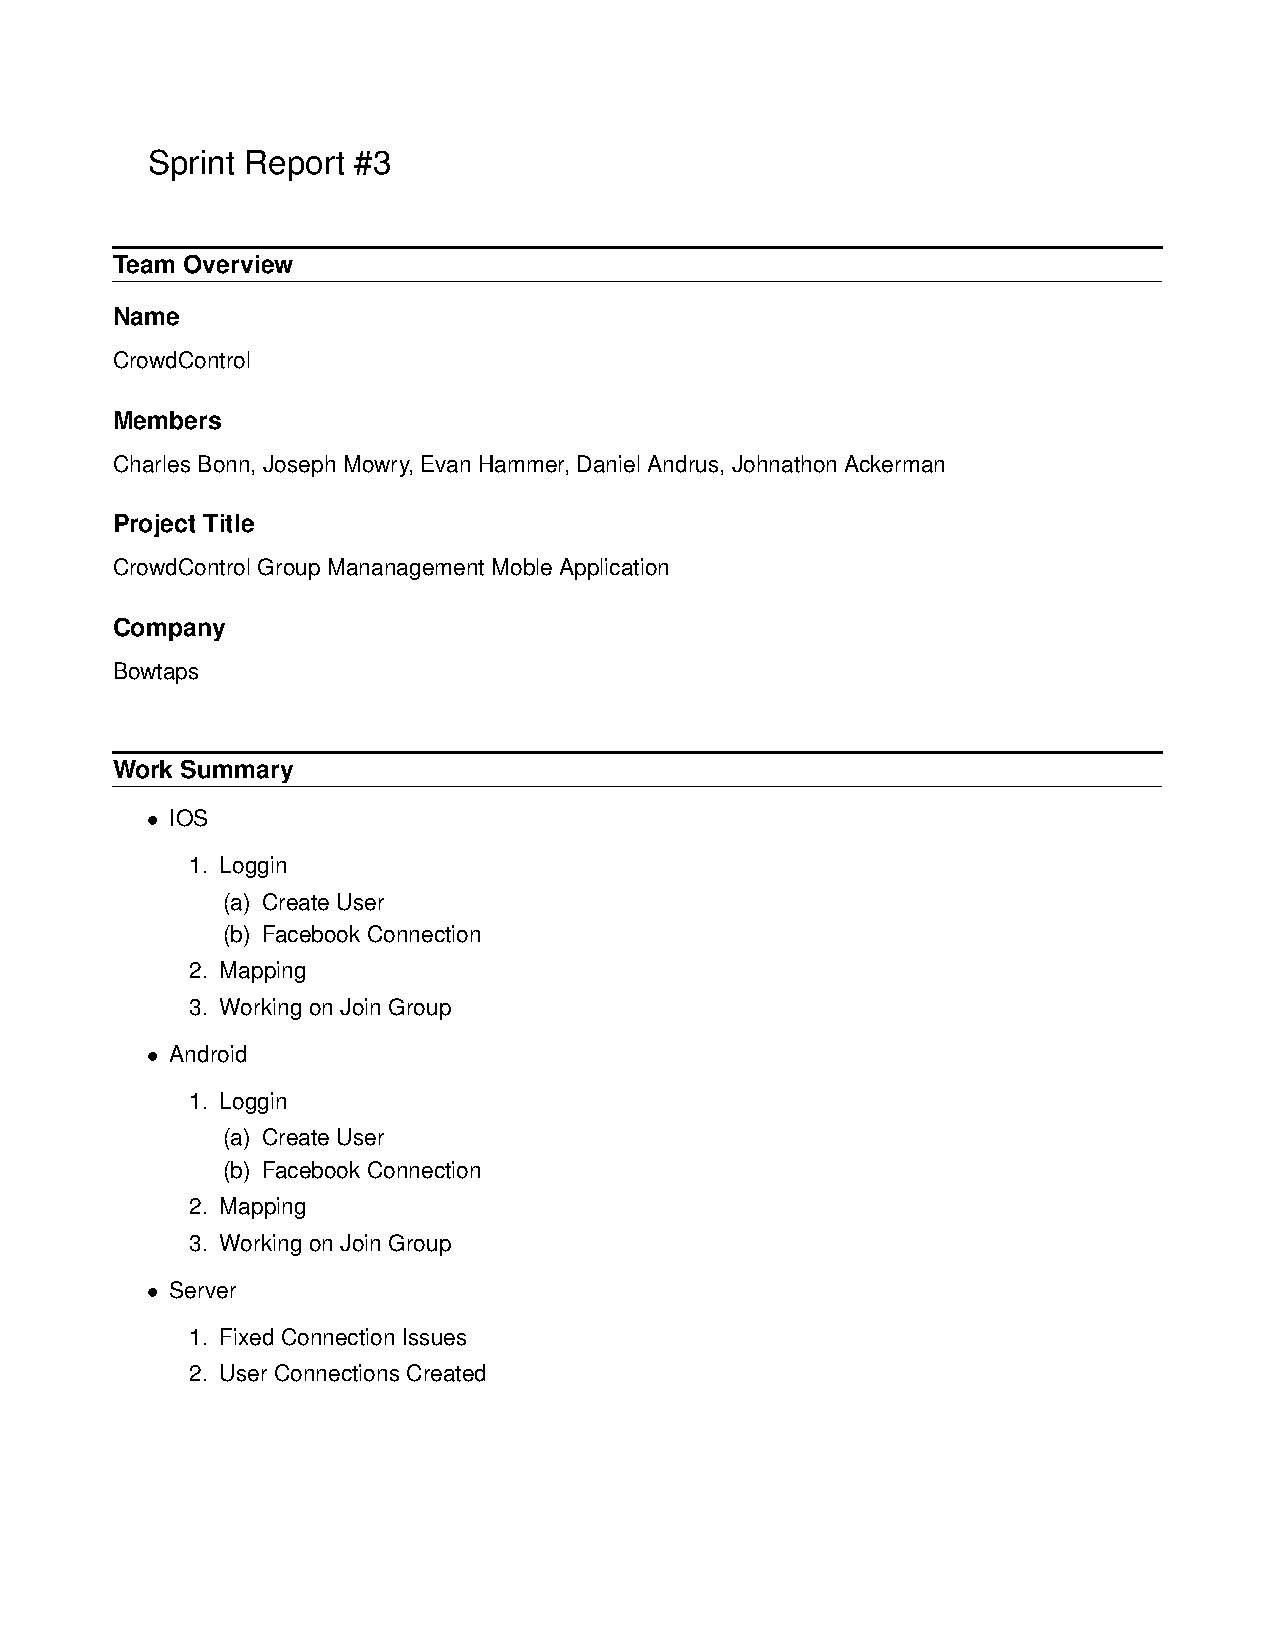
\includepdf[pages=-]{Additional/sprints/sprint3_wrapper.pdf}

%\section{Sprint Report Winter Sprint}

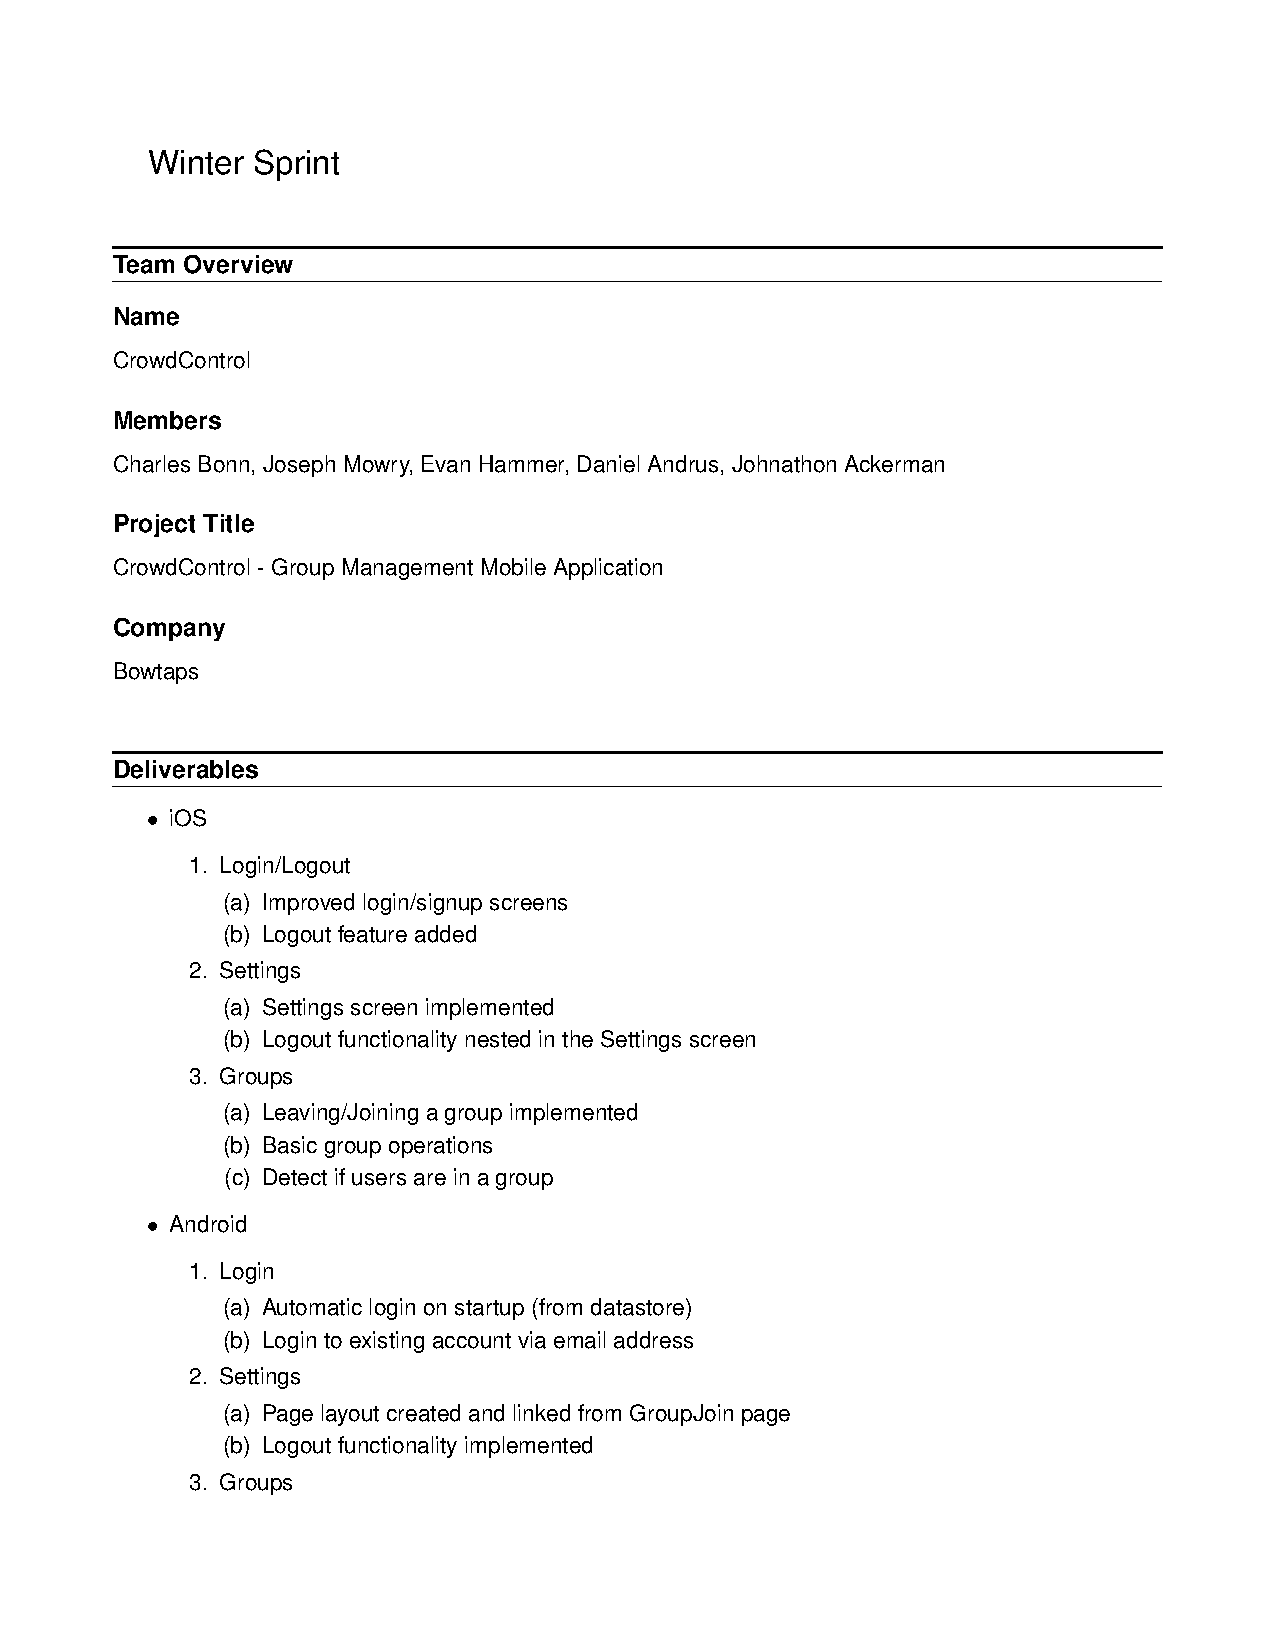
\includepdf[pages=-]{Additional/sprints/wSprintWrapper.pdf}

%\section{Sprint Report Winter Sprint}

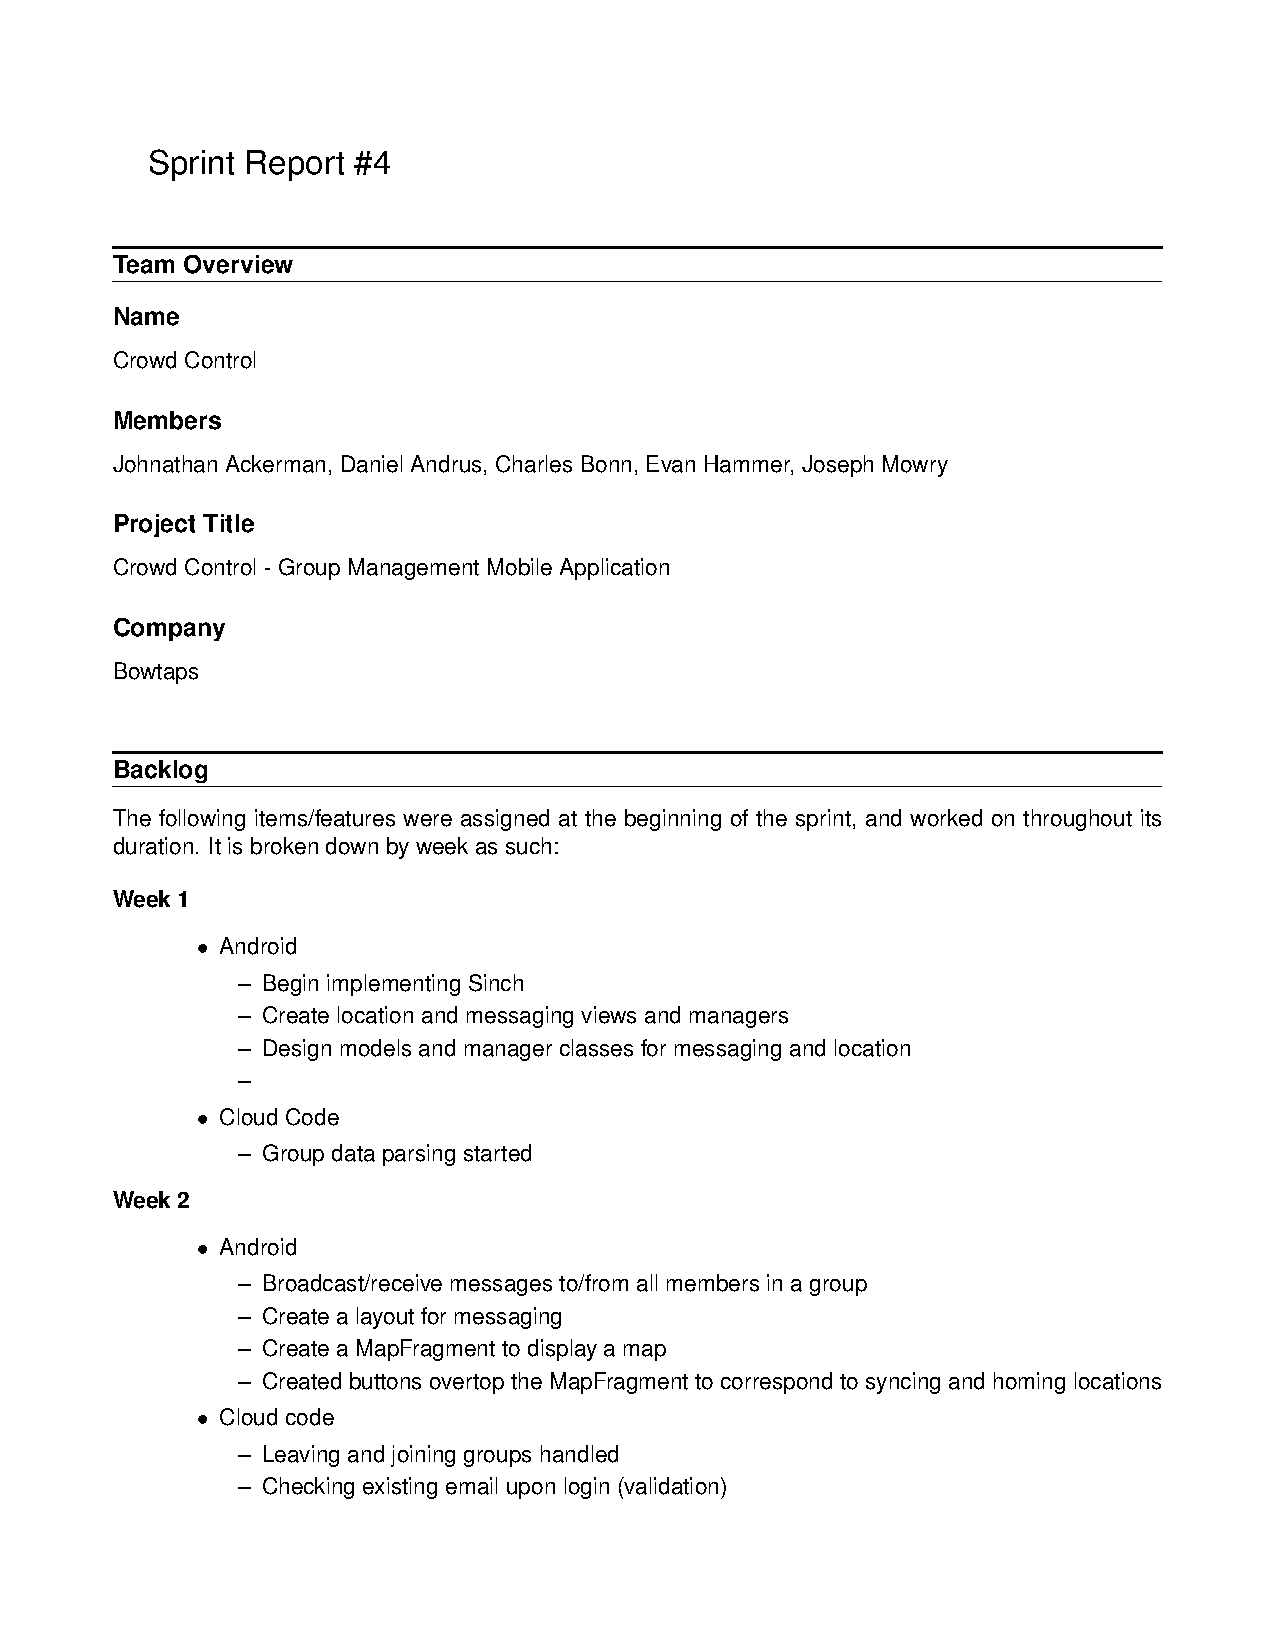
\includepdf[pages=-]{Additional/sprints/Sprint4Wrapper.pdf}



%\chapter{Industrial Experience and Resumes}
%% !TEX root = SystemTemplate.tex


\section{Resumes}

Below are the resumes for the group members: Johnathon Ackerman, Daniel Andrus, Charles Bonn, Evan Hammer, and Joseph Mowry.

%    \includepdf[pages={1}]{report.pdf}  %% example of limited page include

%     \includepdf{resume1.pdf}
%     \includepdf{resume2.pdf}
%     \includepdf{resume3.pdf}
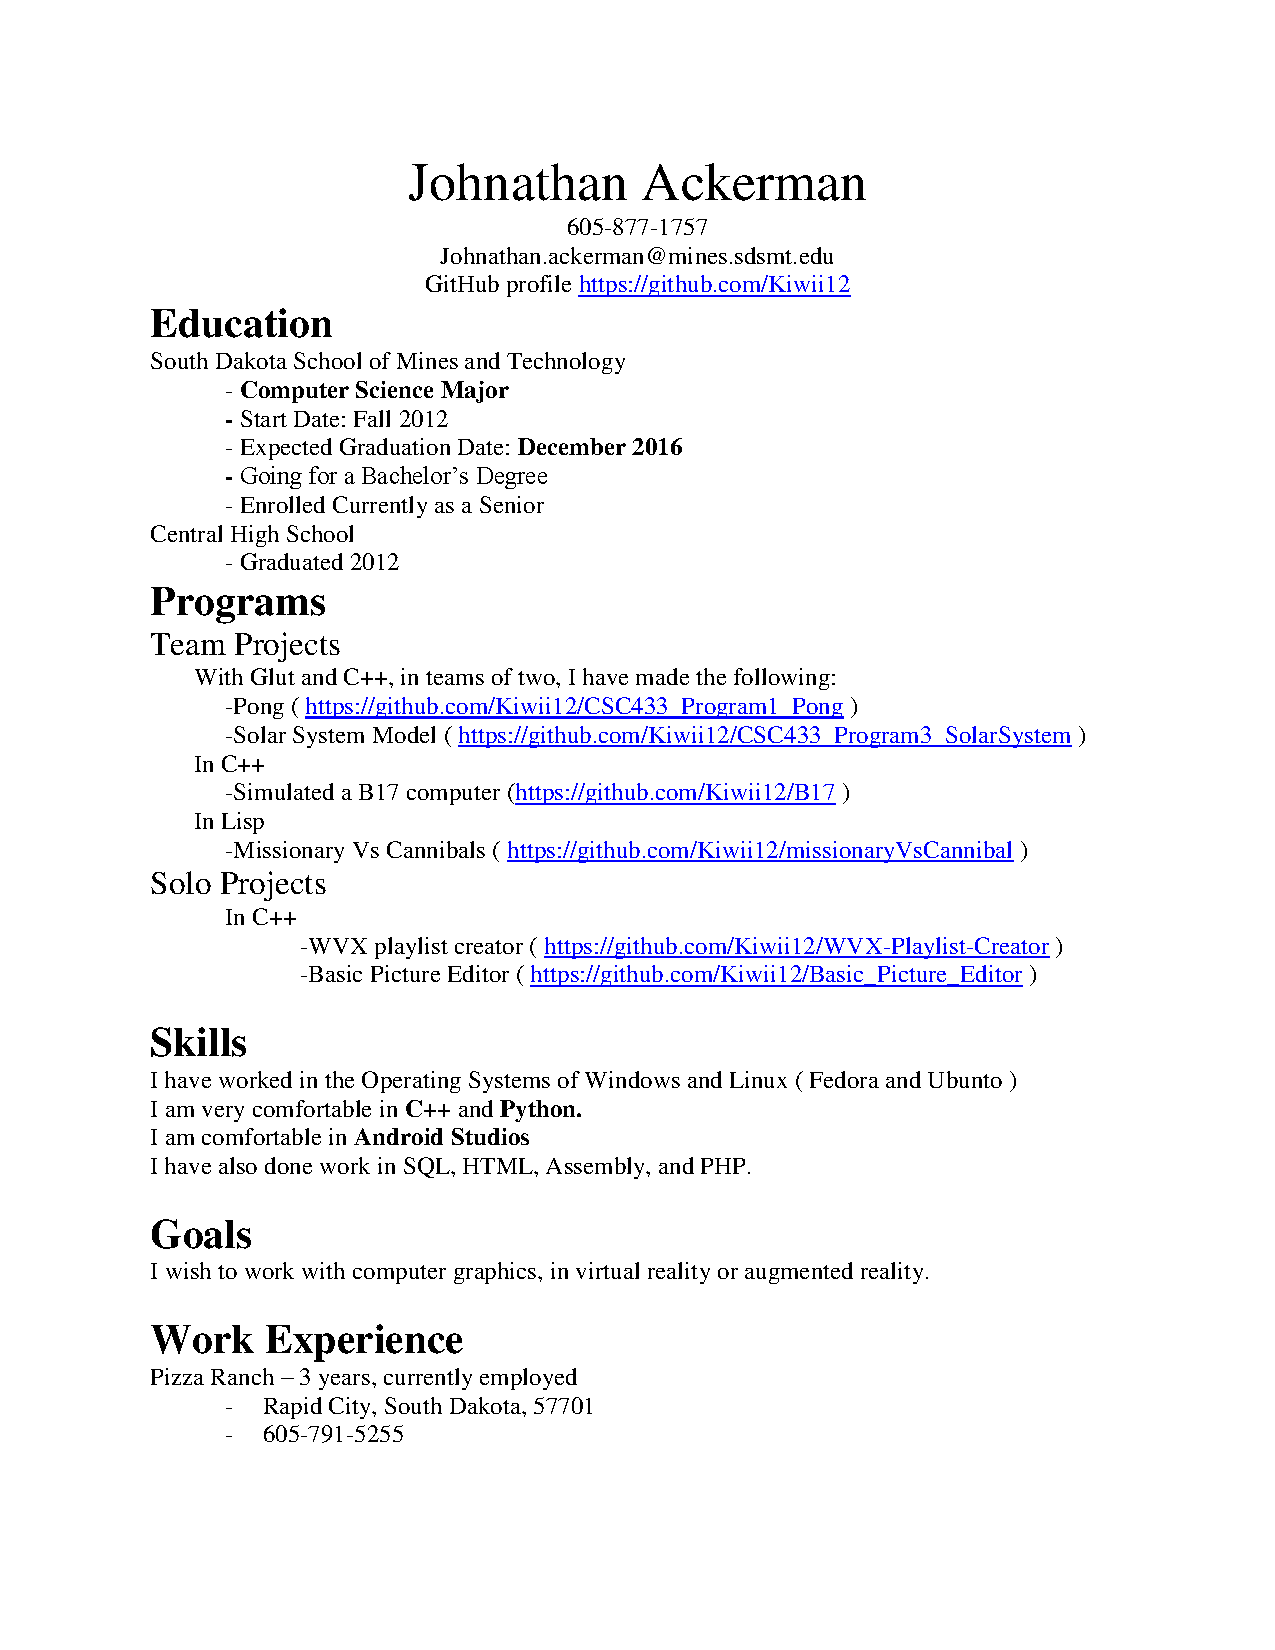
\includepdf{resumes/JohnathonAckermanResume.pdf}
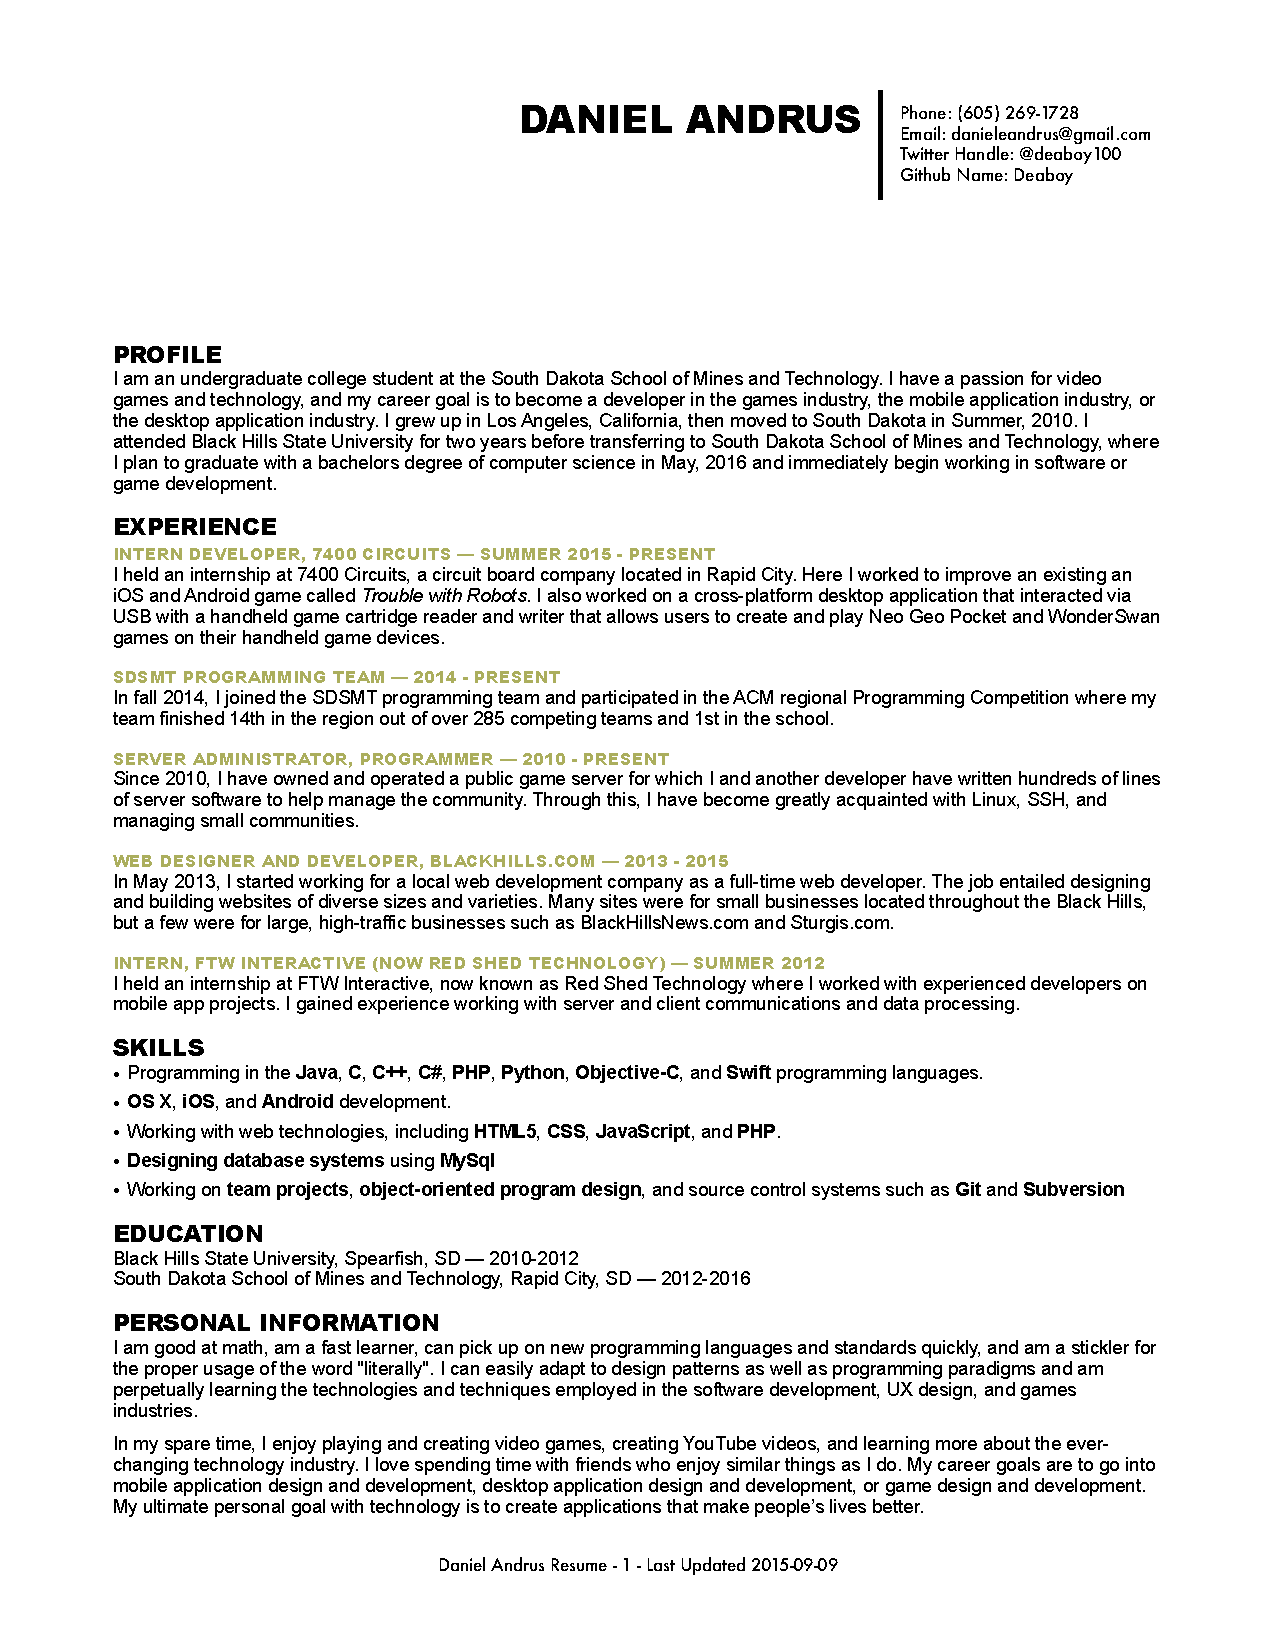
\includepdf{resumes/DanAndrusResume.pdf}
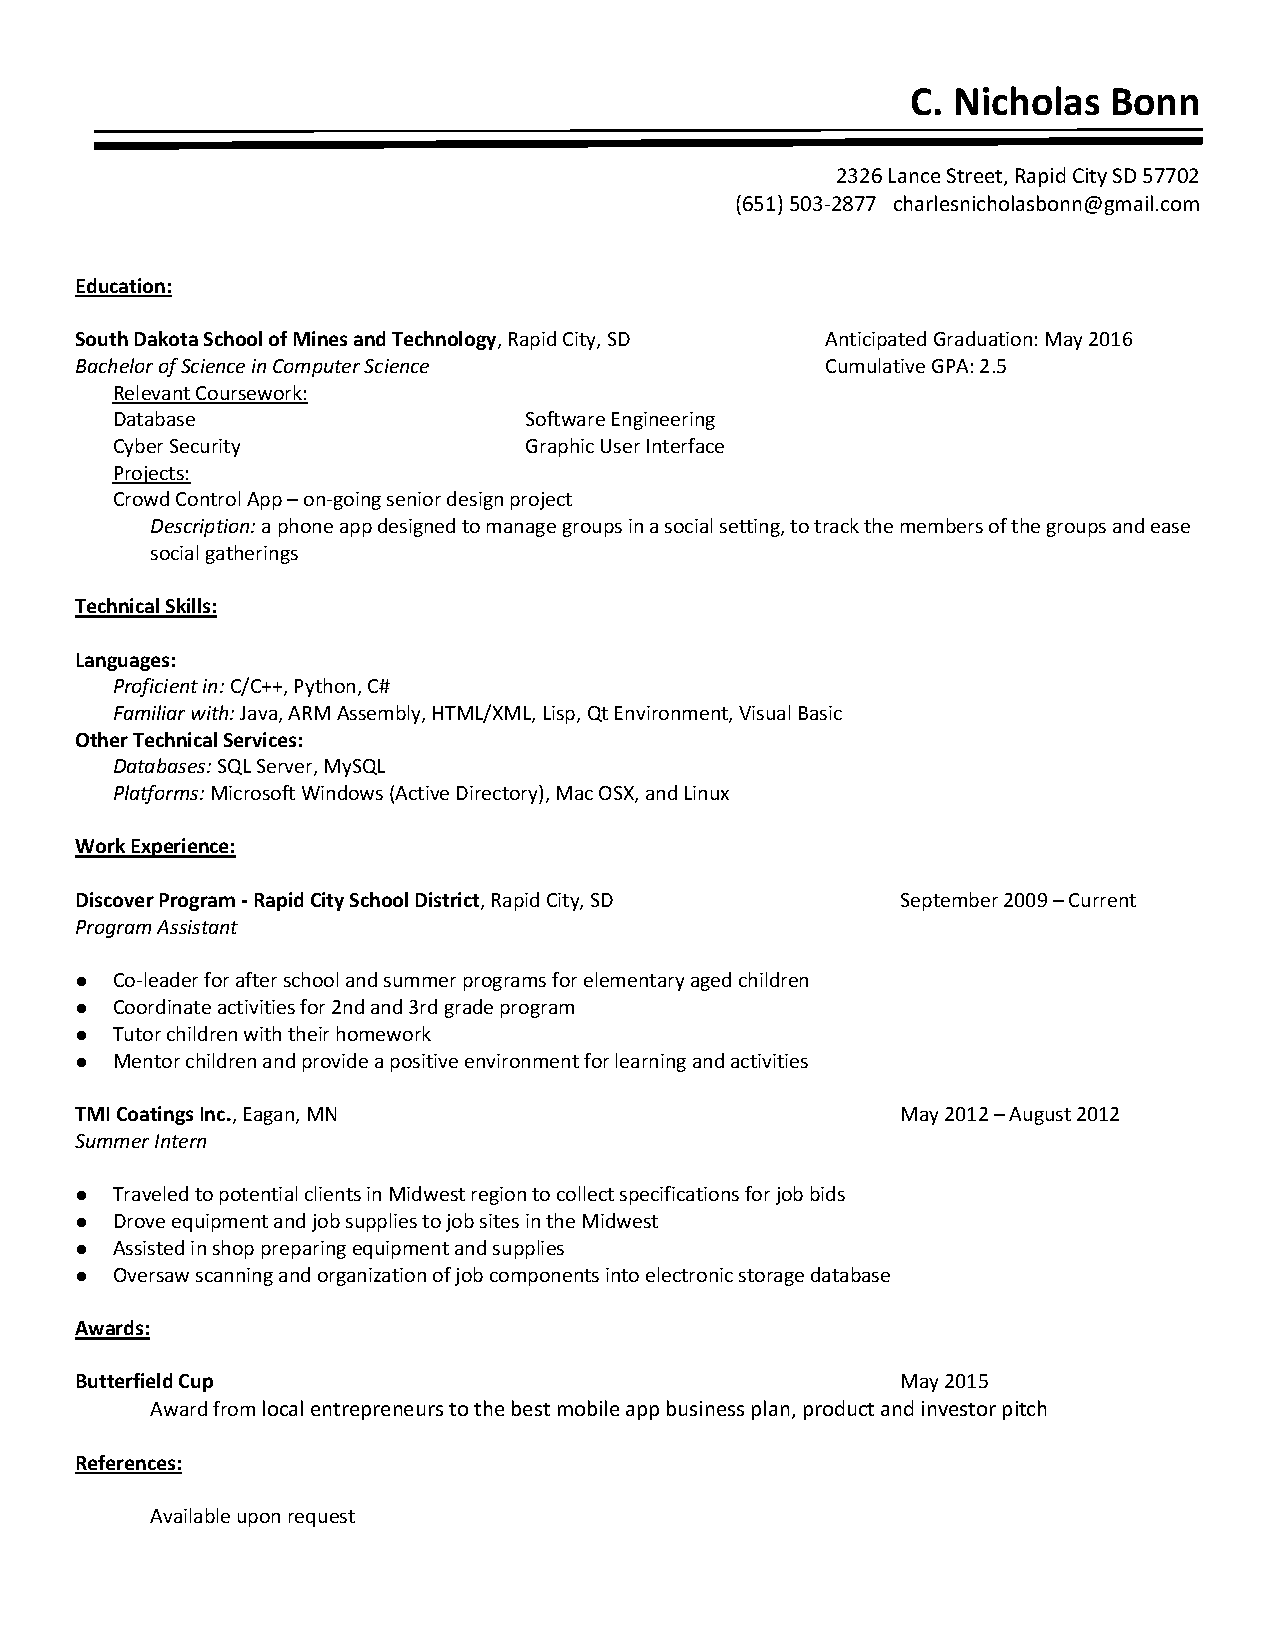
\includepdf{resumes/NickBonnResume.pdf}
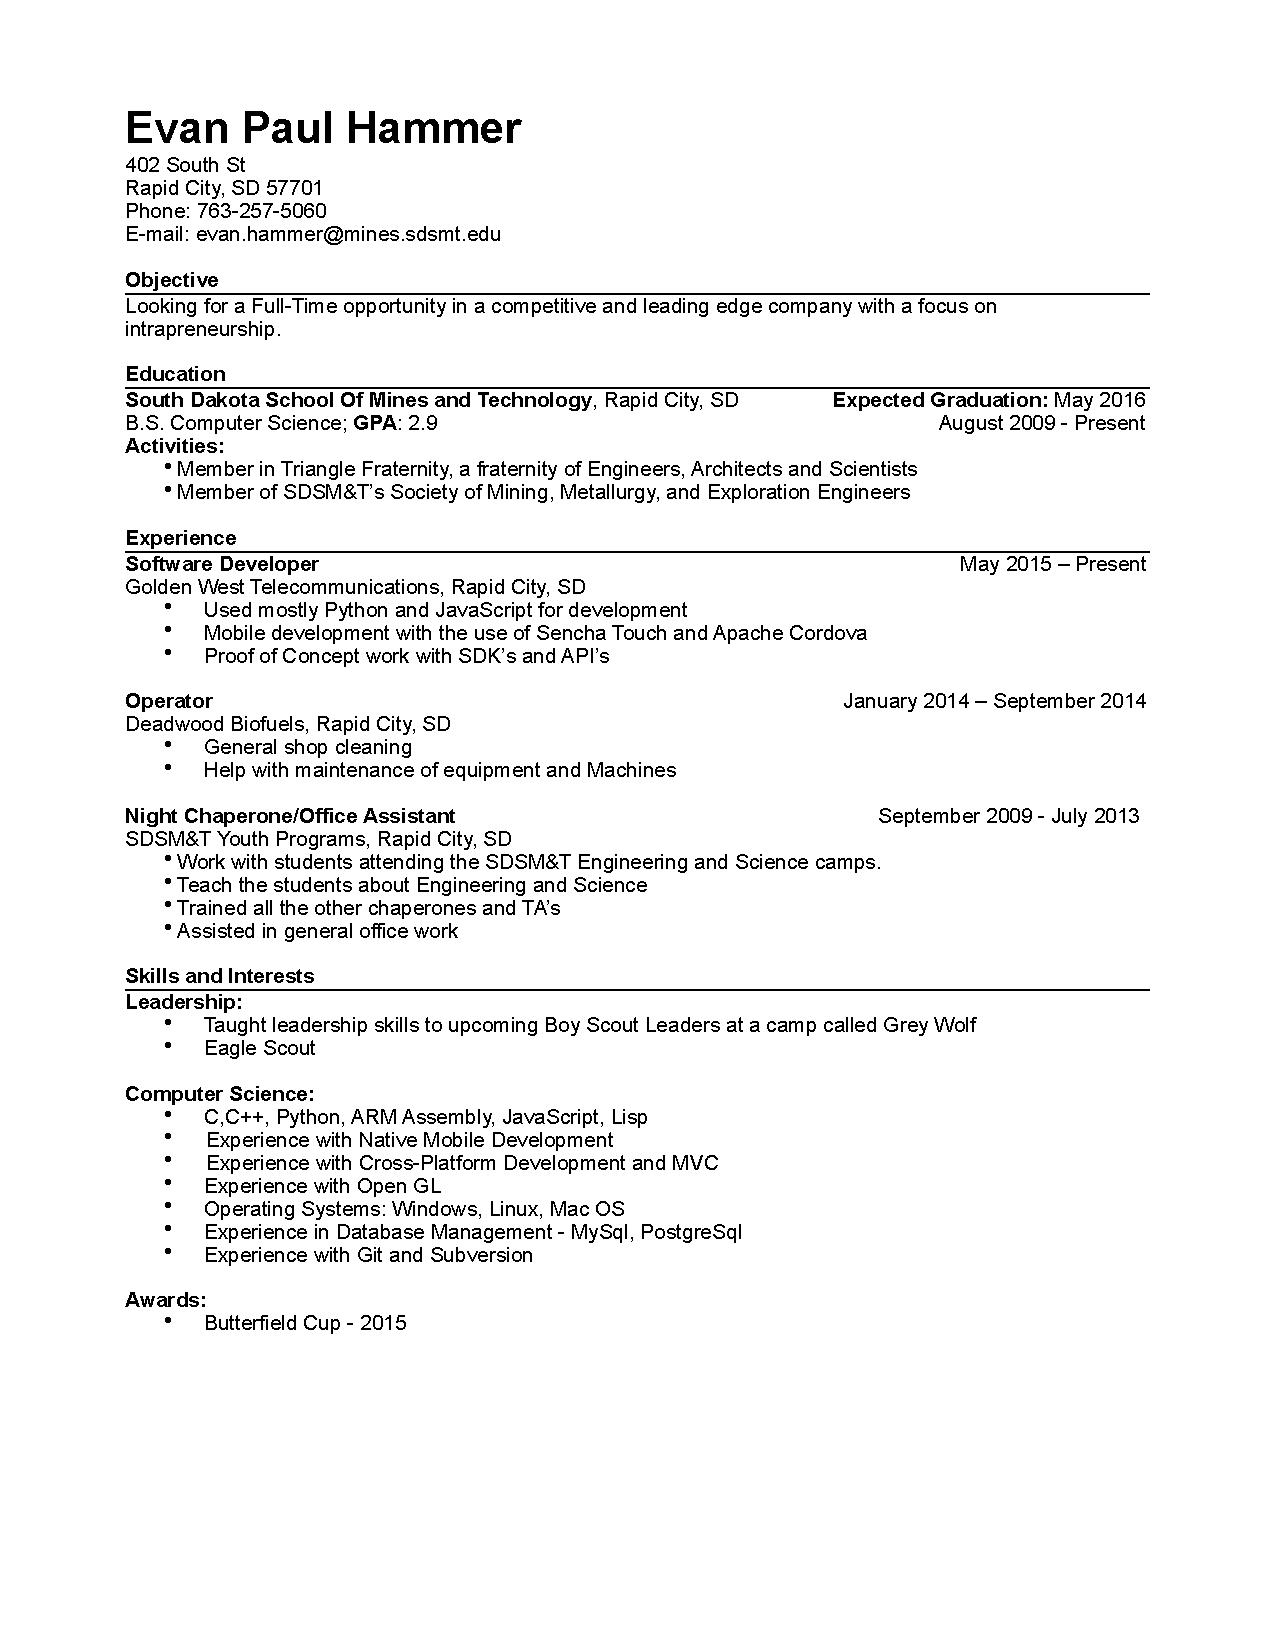
\includepdf{resumes/EvanHammerResume.pdf}
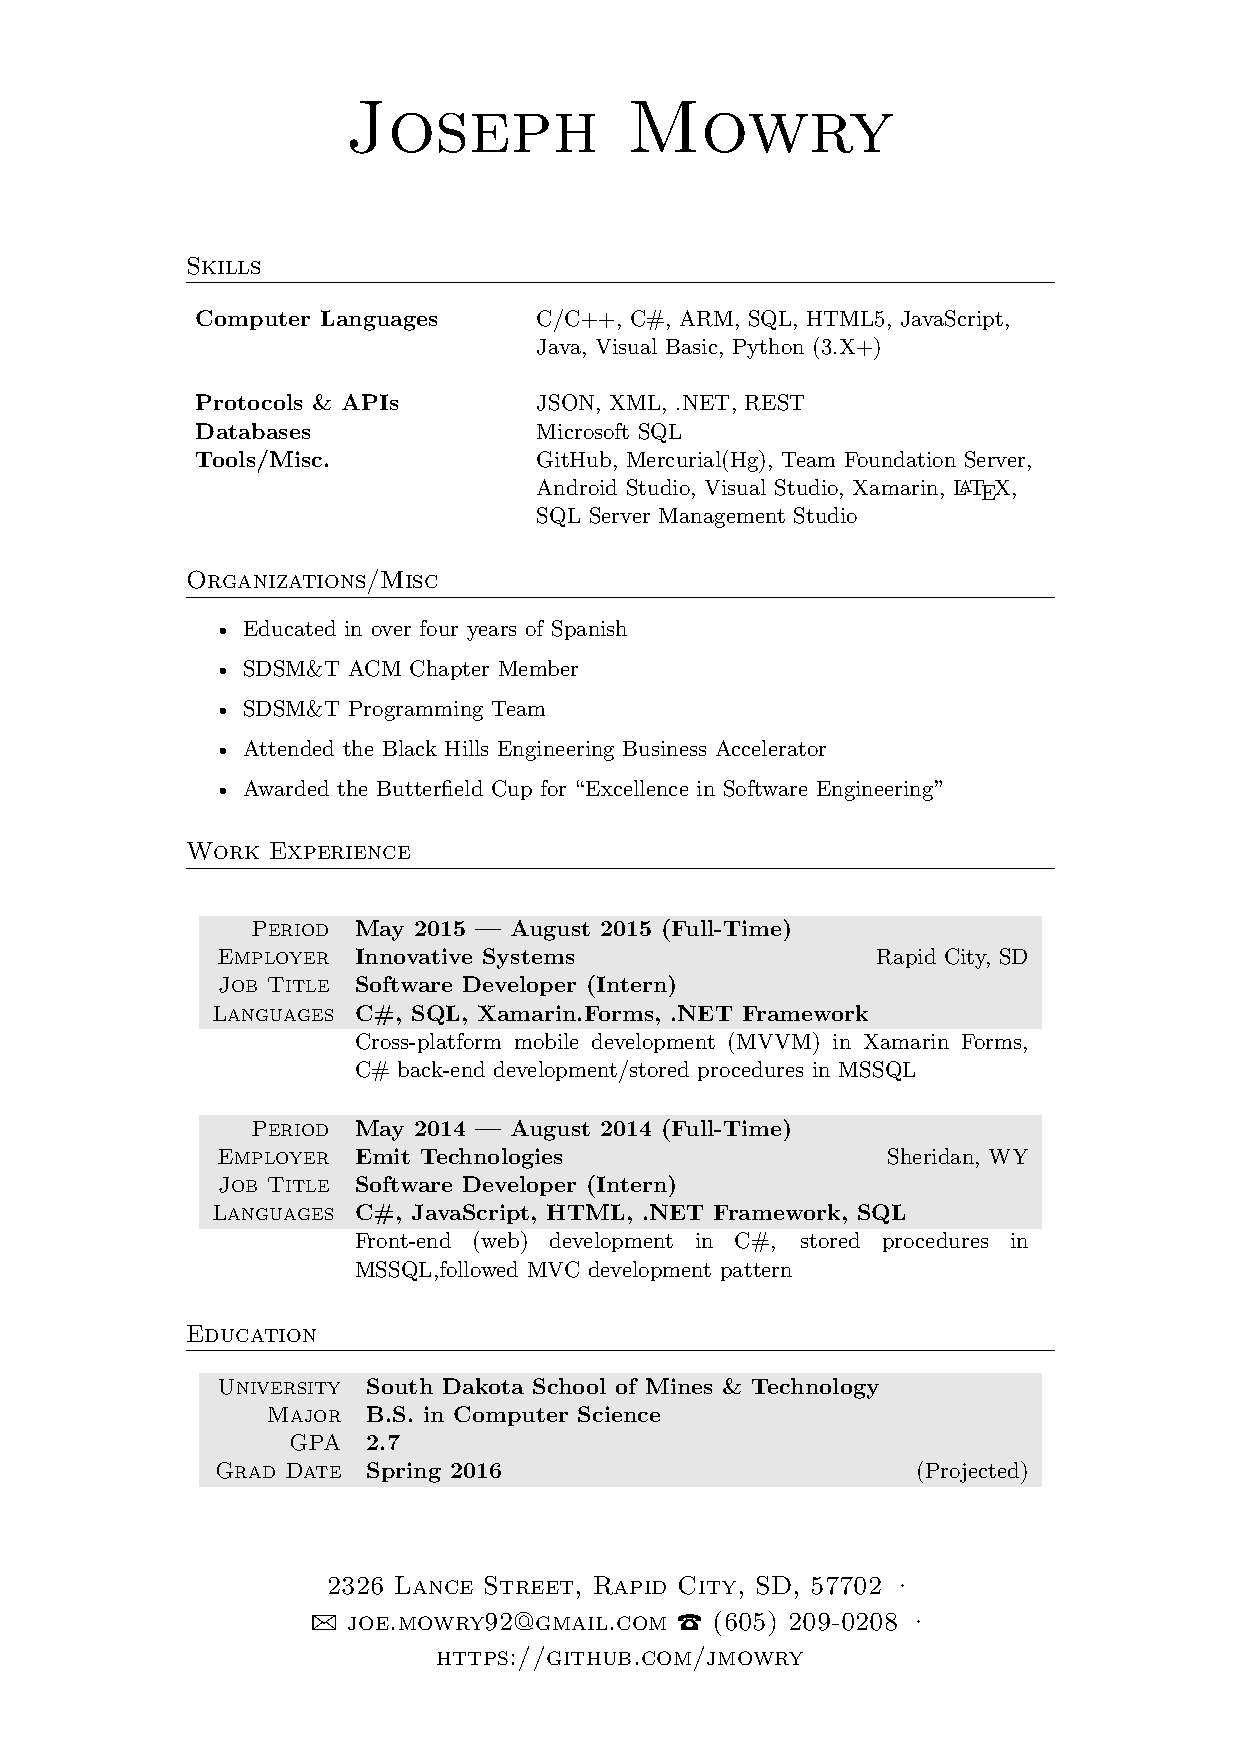
\includepdf{resumes/JosephMowryResume.pdf}

\section{ABET:  Industrial Experience Reports}
As a group we have attended the  SD Engineering Accelerator. We have compeated in multiple business plan competitions including:
	\begin{itemize}
	\item{Butterfield Cup}
	\item{SD Innovation Expo Business Plan Competition}
	\item{2015 SD Mines CEO Student Business Plan Competition}
	\end{itemize}
We also have also have and regular meetings with SDSMT EIR's to help format our buisness plan and Crowd Control.

\subsection{Johnathon Ackerman}

 I have had no Internship experience. However, before the project Crowd Control, I worked with C++, lisp, and python. I have worked with Visual Studios on Windows side, and Vim and G edit in Linux. 

\subsection{Daniel Andrus}

I first learned the basics of web design and development in high school. After my second year of college, I obtained an internship with FTW Interactive (now known as Red Shed Technologies). Later, I hold a position as Web Developer for 2 years before becoming an intern software developer at 7400 Circuits.

My course experience has ranged from data structures, image processing, database design, web development, group projects, computer graphics (including 3D graphics), mobile app development, and even compression.

\subsection{Charles Bonn}

I currently have little internship experence. What industry experence i do have is HTML. In my personal/professional life i help manage a website and a minecraft server. Though this is work i have worked with HTML and C code. I have also worked with game code that is java based.

\subsection{Evan Hammer}

I am working for Golden West Telecommunications(GW), a rural telecommunications provider in the state of South Dakota.  Since May of 2015 I have been a Software Developer for GW working on both mobile and back-end products.  For the mobile side, I have been working with a product called Cordova that is wrapped with another product called Sencha Touch.  Together these two products allow a developer to use JavaScript, HTML, CSS and more to produce a mobile application for Android, iOS and many other mobile platforms.  I have also written the back-end for this app, using Python and a PostgreSQL Database creating a server-side API for the mobile application.  While I am not working on the mobile application I have spent my time working on other in-house products using languages like Python and JavaScript.  These projects have ranged from updating existing code to ground-up projects.  Also as a Software Developer for GW, I have been tasked with creating some proof of concept work.  This work has ranged from testing possible new services as well as testing new platforms for development.  My work continues to grow and change as I continue to work for Golden West Telecommunications.

\subsection{Joseph Mowry}

In his pirior industry experience, Joseph specialized in C\# development and database management. His employers gave him a solid footing in AGILE and Scrum methodologies, as well as general product development. Though his experience lies primarily on the Visual Studio/C\# side of things, there is a large amount of skill overlap in Android Studio and Java that he can bring to the table for this project.




%\chapter{Acknowledgment}
%\label{SpecialThanks}  
%Thanks  

%\chapter{Supporting Materials}
%
This document will contain several appendices used as a way to separate out major 
component details, logic details, or tables of information.  Use of this structure 
will help keep the document clean, readable, and organized. 



% chapters in backmatter don't have numbers, but they appear in the
% table of contents, and are numbered BM-X where X is the page number
% relative to where the backmatter begins.
\backmatter

%% Example
%\chapter{Course Syllabus}
%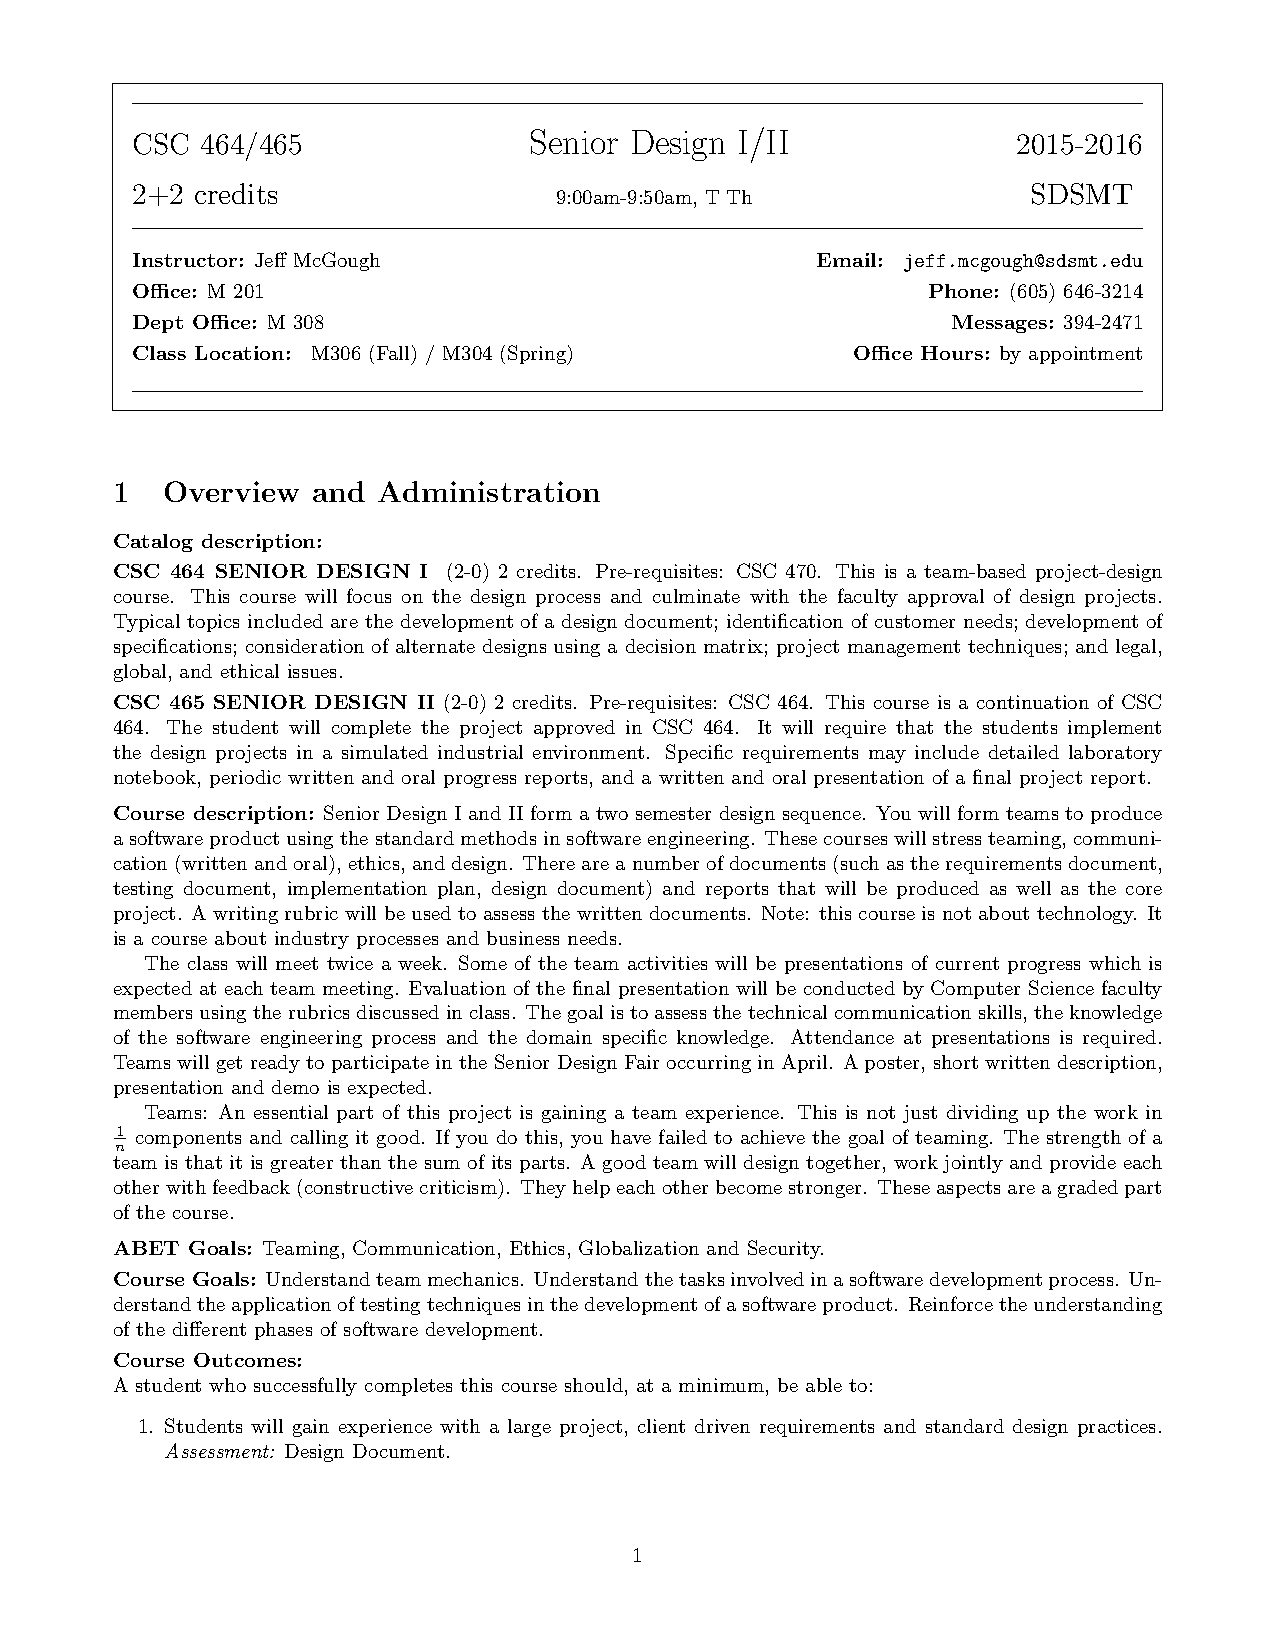
\includepdf[pages={1-17}]{syllabus.pdf}

%%% Remove after reading
%\chapter{\LaTeX\ Example}
%% !TEX root = SystemTemplate.tex


\LaTeX\xspace sample file:  {\color{red} Remove from submitted materials}

\section{Introduction}
This is a sample input file.  Comparing it with the output it
generates can show you how to produce a simple document of
your own.

\section{Ordinary Text}  % Produces section heading.  Lower-level
                                    % sections are begun with similar 
                                    % \subsection and \subsubsection commands.

The ends  of words and sentences are marked 
  by   spaces. It  doesn't matter how many 
spaces    you type; one is as good as 100.  The
end of   a line counts as a space.

One   or more   blank lines denote the  end 
of  a paragraph.  

Since any number of consecutive spaces are treated like a single
one, the formatting of the input file makes no difference to
      \TeX,         % The \TeX command generates the TeX logo.
but it makes a difference to you.  
When you use
      \LaTeX,       % The \LaTeX command generates the LaTeX logo.
making your input file as easy to read as possible
will be a great help as you write your document and when you
change it.  This sample file shows how you can add comments to
your own input file.

Because printing is different from typewriting, there are a 
number of things that you have to do differently when preparing 
an input file than if you were just typing the document directly.  
Quotation marks like 
       ``this'' 
have to be handled specially, as do quotes within quotes: 
       ``\,`this'                  % \, separates the double and single quote.
        is what I just 
        wrote, not  `that'\,''.  

Dashes come in three sizes: an 
       intra-word 
dash, a medium dash for number ranges like 
       1--2, 
and a punctuation 
       dash---like 
this.

A sentence-ending space should be larger than the space between words
within a sentence.  You sometimes have to type special commands in
conjunction with punctuation characters to get this right, as in the
following sentence.
       Gnats, gnus, etc.\    % `\ ' makes an inter-word space.
       all begin with G\@.   % \@ marks end-of-sentence punctuation.
You should check the spaces after periods when reading your output to
make sure you haven't forgotten any special cases.
Generating an ellipsis 
       \ldots\    % `\ ' needed because TeX ignores spaces after 
                  % command names like \ldots made from \ + letters.
                  %
                  % Note how a `%' character causes TeX to ignore the 
                  % end of the input line, so these blank lines do not
                  % start a new paragraph.
with the right spacing around the periods 
requires a special  command.  

\TeX\ interprets some common characters as commands, so you must type
special commands to generate them.  These characters include the
following: 
       \$ \& \% \# \{ and \}.

In printing, text is emphasized by using an
       {\em italic\/}  % The \/ command produces the tiny extra space that
                       % should be added between a slanted and a following
                       % unslanted letter.
type style.  

\begin{em}
   A long segment of text can also be emphasized in this way.  Text within
   such a segment given additional emphasis 
          with\/ {\em Roman} 
   type.  Italic type loses its ability to emphasize and become simply
   distracting when used excessively.  
\end{em}

It is sometimes necessary to prevent \TeX\ from breaking a line where
it might otherwise do so.  This may be at a space, as between the
``Mr.'' and ``Jones'' in
       ``Mr.~Jones'',        % ~ produces an unbreakable interword space.
or within a word---especially when the word is a symbol like
       \mbox{\em itemnum\/} 
that makes little sense when hyphenated across 
       lines.

Footnotes\footnote{This is an example of a footnote.}
pose no problem.

\TeX\ is good at typesetting mathematical formulas like
       \( x-3y = 7 \) 
or
       \( a_{1} > x^{2n} / y^{2n} > x' \).
Remember that a letter like
       $x$        % $ ... $  and  \( ... \)  are equivalent
is a formula when it denotes a mathematical symbol, and should
be treated as one.

\section{Displayed Text}

Text is displayed by indenting it from the left margin.
Quotations are commonly displayed.  There are short quotations
\begin{quote}
   This is a short a quotation.  It consists of a 
   single paragraph of text.  There is no paragraph
   indentation.
\end{quote}
and longer ones.
\begin{quotation}
   This is a longer quotation.  It consists of two paragraphs
   of text.  The beginning of each paragraph is indicated
   by an extra indentation.

   This is the second paragraph of the quotation.  It is just
   as dull as the first paragraph.
\end{quotation}
Another frequently-displayed structure is a list.
The following is an example of an {\em itemized} list.
\begin{itemize}
   \item  This is the first item of an itemized list.  Each item 
          in the list is marked with a ``tick''.  The document
          style determines what kind of tick mark is used.

   \item  This is the second item of the list.  It contains another
          list nested inside it.  The inner list is an {\em enumerated}
          list.
          \begin{enumerate}
              \item This is the first item of an enumerated list that
                    is nested within the itemized list.

              \item This is the second item of the inner list.  \LaTeX\
                    allows you to nest lists deeper than you really should.
          \end{enumerate}
          This is the rest of the second item of the outer list.  It
          is no more interesting than any other part of the item.
   \item  This is the third item of the list.
\end{itemize}
You can even display poetry.
\begin{verse}
   There is an environment for verse \\    % The \\ command separates lines
   Whose features some poets will curse.   % within a stanza.

                           % One or more blank lines separate stanzas.

   For instead of making\\
   Them do {\em all\/} line breaking, \\
   It allows them to put too many words on a line when they'd 
   rather be forced to be terse.
\end{verse}

Mathematical formulas may also be displayed.  A displayed formula is
one-line long; multi-line formulas require special formatting
instructions.
   \[  x' + y^{2} = z_{i}^{2}\]
Don't start a paragraph with a displayed equation, nor make
one a paragraph by itself.

\section{Build process}

To build \LaTeX\ documents you need the latex program.  It is free and available on all operating systems.   Download and install.  Many of us use the TexLive distribution and are very happy with it.    You can use a editor and command line or use an IDE.  To build this document via command line:

\begin{verbatim}
alta>  pdflatex SystemTemplate
\end{verbatim}
If you change the bib entries, then you need to update the bib files:
\begin{verbatim}
alta>  pdflatex SystemTemplate
alta>  bibtex SystemTemplate
alta>  pdflatex SystemTemplate
alta>  pdflatex SystemTemplate
\end{verbatim}

The template files provided also contain a Makefile, which will
make things much easier.  

\section*{Acknowledgment}
Thanks to Leslie Lamport.  






\end{document}
